 \ifdefined\FromMain %
 \else % 
 	\documentclass[../main.tex]{subfiles}
 	\let\FromMain\undefined
   	\begin{document}
 \fi


\chapter{Modèle numérique du métabolisme bactérien de la production d'un fromage}
\label{tango}
\minitoc
Soumis dans metabolic engineering 

\doublespacing %% For correction

\newpage

Les données multi-omiques permettent une comprehension du métabolisme à différents niveaux que sont: métatranscriptomiques, l'étude de l'expression de tous les gènes d'une communauté données; métabolomiques, l'étude de l'ensemble des métabolites; génomiques; les génomes de chaque souche bactérienne. Dans ce chapitre nous verrons comment les données omiques, le paramétrage de chaque souche bactérienne ainsi qu'un partage équilibré des ressources pour chaque membre de la communauté permet d'obtenir un modèle numérique de la fermentation bactérienne d'un fromage modèle précis mettant en avant des interactions bactériennes. 

\section{Introduction}

La fermentation des aliments et des boissons par un consortium bactérien compte parmi les plus vieux processus technologiques alimentaires, associés aux bénéfices alimentaires et utilisés aujourd'hui à la fois dans les contextes traditionnels et industriels \citep*{Tamang2016,Tamang.2016_Functional}. La transformation alimentaire par les micro-organismes est le résultat de processus métaboliques et d'interactions entre les membres de la communauté bactérienne. Cette dernière peut être contrôlé, comme c'est le cas dans les processus industriels \citep{Somerville.2021}, afin de garantir des produits alimentaires sains et prévoir des propriétés organoleptiques \citep{Galimberti.2021}. Au sein de communautés, les propriétés fonctionnelles des souches bactériennes associées au produits fermentés sont mieux compris \citep{Tamang.2016_Functional}, en revanche, les mécanismes moléculaires précis mis en jeu commencent seulement à être explorés \citep{Blasche.2021}. En effet, la compréhension du métabolisme individuel des membres d'un consortium n'est pas suffisante pour capturer ou prédire les comportement globaux de la communauté, qui est impacté par les interactions microbe-microbe.

Un moyen pour caractériser toutes les fonctions et les interaction d'un consortium microbien de produits fermentés est de combiner les approches en biologie des systèmes avec les données omiques \citep{Mannaa.2021}. Un première approche consiste à procéder à l'inventaire des métabolites et espèces d'une communauté via des méthodes de cultures dépendants ou indépendants\citep{Blasche.2021}. Dans le cas d'une communauté contrôlée, une comparaison en mono et en co-cultures peut nous informer sur, l'impact des interactions, sur la dynamique et sur les profiles métaboliques de la communauté \citep{Ozcan.2020}. Du point de vue des méthodes non culture-dépendantes, l'utilisation de modèles métaboliques à l'échelle du génome (GEMs) \citep{Fang.2020} semble particulièrement opportun comme un moyen d'associer les souches du consortium à la fonction porté par les systèmes et à termes aux propriétés organoleptiques alimentaires \citep{Ozcan.2020}. Ces modèles de consortium bactérien sont utilisables pour un grand nombre d'application comme dans les biotechnologies alimentaires, allant de l'assemblage de souches dans la création de communautés à l'optimisation de procédés pour les propriétés organoleptiques désirées \citep{Rau.2018}.

L'analyse de consortia bactérien permet difficilement la construction de modèle mécanistique ou d'un jumeau numérique de part la complexité de la communauté bactérienne, ainsi que la grande spécificité souches-dépendantes des voies métaboliques secondaires impliqué dans les processus organoleptiques. Ainsi, travailler à petite échelle avec des systèmes contrôlés où la complexité est réduite semble être particulièrement pertinent \citep{Rau.2018}. Actuellement, même sur des systèmes simples une modélisation temporelle peut être pris en compte, comme c'est le cas pour la fermentation qui est un processus dynamique. 


Dans ce chapitre, nous vous présenterons un modèle simplifié de la fabrication du fromage, à partir des éléments nutritifs du lait jusqu'à l'étape d'affinage. Ce modèle se concentre sur le métabolisme d'une communauté bactérienne composés de deux bactéries lactiques (LAB) \textit{Lactococcus lactis}, \textit{Lactiplantibacillus plantarum} et d'une bactéries propionique \textit{Propionibacterium freudenreichii} permettant de la production de fromage industriel. Nous nous sommes basés sur les travaux de \citep{Cao2021}, décrivant comment le paramétrage d'un processus standardisé de fabrication d'un fromage peut moduler la production de composés aromatiques. Pour cela, les réseaux métaboliques à l'échelle du génome ainsi que le modèle communautaire fut construit et exploité grâce au données omiques dans le but de (i) évaluer la contribution métabolique de chaque espèce microbienne durant la fabrication de fromage, (ii) de simuler les dynamiques des métabolismes microbiens ainsi que l'effet de la communauté sur le comportement des individus et enfin (iii) proposer des interactions possibles entre les espèces bactériennes.

La méthode consiste à identifier les chemin métaboliques responsables de la transformation des nutriement présent initialement dans le lait. Nous avons par la suite optimisé chacun de nos modèles métaboliques individuels afin d'être capable de reproduire la dynamique des cultures pures. Enfin, ces modèles individuels sont utilisés pour construire un modèle dynamique de la communauté prédisant avec précision la production de composés aromatiques du fromage.

\section{Résultats}
\subsection{Les modèles métaboliques individuels identifient des voies métaboliques spécifiques dans le lait}
Dans cette première sous-section, nous nous focaliserons sur le processus d'affinage des modèles de flux individuels de chaque espèce. En effet, l'hypothèse que nous explorons consiste à suffisamment nettoyer les réseaux métaboliques à l'échelle du génome pour construire un modèle numérique de la communauté capable de caractériser une communauté bactérienne à la fois sur le plan des interactions bactériennes et à la fois sur des biens métaboliques. Pour cela, nous avons commencé par une étude comparative des génomes ainsi que des réseaux métabolique à l'échelle du génome afin de vérifier la qualité topologique des réseaux. Dans un second temps, nous avons examiné le métabolisme carboné central de chaque souche en prêtant une attention particulière au métabolisme secondaire dans le but de vérifier la production et la consommation de certains métabolites se fait par les bonnes voies métaboliques. Enfin, dans le but de obtenir des valeurs de biomasse, de production et de consommation numériquement proches des observations biologiques, une étape d'inférence de paramètres a été faite souche dépendante. \\

La communauté bactérienne étudiée est composé de \textit{Propionibacterium freudenreichii} CIRM-BIA122, \textit{Lactiplantibacillus plantarum} CIRMB-BIA465 et de \textit{Lactococcus lactis} biovar \textit{diacetyl lactis}. Pour chacun d'entre eux, le longueur total de l'ADN a été récupéré et les génomes bactériens ont été assemblés à partir d'une combinaison de lectures courtes et longues, produisant un assemblage précis et complet. Cet assemblage a révélé un chromosome circulaire et la présence de sept plasmides pour la souche de \lactis et quatre plasmides pour la souche de \plantarum. Parmi ce consortium bactérien seul la souche de \freud ne porte pas de plasmide. Une annotation du génome a été faite et déposé sous le numero d'accesion ENA suivant : ENA: PRJEB42478. L'annotation a identifié une liste de 8234 séquences codantes incluant ceux du chromosome (2460 pour \freud, 2417 for \lactis et 3016 pour \plantarum) et des plasmides (139 pour \lactis et 82 pour \plantarum). D'autres informations telles que le nombre de gênes codant pour des protéines, de séquences ribosomiques, tRNA et le pourcentage de GC sont rassemblés dans la Table \ref{tab:genomes}.\\

Les réseaux métaboliques à l'échelle du génomes ont été reconstruit pour chaque souche individuelle depuis leurs séquences génomiques annotées respectives. Après une première étape automatique de reconstruction, nous avons réalisé un raffinement manuel du métabolisme carboné central basé sur la litérature et la connaissance biologique dans le but de prendre en compte la specificité de chaque souche bactérienne. La qualité de chaque réseau métabolique a été vérifié et répond aux attendus : une faible fraction de réactions universellement bloqués (< 3\%), et une faible fraction de réaction sans association de gène-proteine-réactions (GPR) (< 30\%) \citep{Lieven.2020}. La Table \ref{tab:table1} décrit les caractéristiques des trois modèles et nous observons que \lactis a le plus petit nombre de réactions que les deux autres souches, une différence qualitative qui est aussi observée pour les autres souches de la même espèces dans d'autres bases de données \citep{Noronha.2018}.\\

Nous avons construit les réseaux métaboliques à l'échelle de chaque génome (GEMs) les avons analysés par la méthode d'équilibre des flux (FBA) \citep{Palsson1994,Orth2010} assurant ainsi la production des molécules de la biomasse à partir de l'environnement nutritionnel du lait (voir Materiels et méthodes). Nous avons obtenu des taux de croissances allant de 0.187 $\text{mmol.gDW}^{-1}\text{.hr}^{-1}$ à 2.17 $\text{mmol.gDW}^{-1}\text{.hr}^{-1}$, où le premier est obtenu par \freud et la plus haute valeur obtenu par \lactis. Comme les conditions dans le fromage correspondent à des conditions microaérobiques \citep{Miyoshi2003}, une attention particulière a été donné sur le rôle de l'oxygène sur le métabolisme des trois bactéries en modifiant la borne supérieur de la réaction d'importation dans le compartiment cytosolique.

Le métabolisme carboné central produit du NADH and NADPH et ses formes réduites correspondantes, de l'ATP et les précurseurs nécessaires pour la biosynthèse des molécules essentielles pour la croissance ainsi que pour l'activité métabolique des cellules bactériennes, e.g. acides aminés, purine, pyrimidine, glycerol-3-phosphate, acides gras, N-acetyl-glucosamine, vitamines. Parmi les voies métaboliques du métabolisme carboné central, la glycolyse et la voie des pentose phosphate sont partagés entre les trois espèces presque à l'identique. Les sources de carbone telles que le lactose, l'acide citrique et l'acide lactique,sont converties en acide pyruvique, qui sera utilisé \textit{via} d'autres voies spécifiques. La spécificité des voies métaboliques de chaque espèce du métabolisme carboné central est représenté par la Figure \ref{figure:metabolic_map}. Dans la suite du chapitre, les caractéristiques de chaque souche métabolique sera étudié afin de justifier le raffinement fait, en se focalisant sur les voies métaboliques secondaires permettant la production de composés organoleptiques.

\subsubsection{Métabolisme des bactéries lactiques}
Les bactéries lactiques \lactis et \plantarum utilisent le lactose et le citrate, les deux principales sources de carbone du lait \citep{Widyastuti2014}. Le lactose, dégradé par l'enzyme de la beta-galactosidase, se transforme en galactose et glucose, où ce dernier alimente la glycolyse. Concernant le galactose et l'acide citrique, leur métabolisme est souche dépendant \citep{Palles1998}. D'un coté, le alactose est convertie en glucose-6-phosphate \textit{via} la voie métabolique de Leloir avant d'entrer dans la glycolyse, et de l'autre l'acide citrique est convertie en pyruvate par l'enzyme de la citrate lysase à travers la production des acides lactiques et citriques \citep{alma991000892589705596}. Du point de vue du métabolisme secondaire, le butanediol et du diacétyle, responsable de la saveur beurré du fromage, est produit chez les deux modèles à partir du pyruvate et est permise grâce à la voie de l'acétolactate. L'ensemble de ces voies métaboliques décrites ci-dessus sont récapitulés dans le Figure \ref{figure:metabolic_map}~a, b). \\

\paragraph{\lactis}

Pour permettre la production de certains composé d'intérêt, comme le butanediol, le GEM a du être manuellement curé (Fig.~ \ref{figure:metabolic_map}~a). Le flux de l'acetoin-dehydrogenase a été bloqué (ACTD2) permettant la production du butanediol, et les bornes de l'acetolactate decarboxylase (ACLDC), acetolactate synthase (ACLS) ont été modifié permettant l'activation de la voie de l'acetolactate, comme retrouvé dans la littérature \citep*{Carroll1999,Swindell1996,Makhlouf2006}. Enfin, la consommation de lactose a été régule en modifiant les bornes de la réaction LACZ qui a permis un flux de production de lactate pour \lactis (Fig.~ \ref{figure:metabolic_map}~a).\\
Pour valider ce modèle, nous avons considéré un exemple d'activation de voie métabolique durant la production du fromage. Il est montré que \lactis consomme le lactose à la fois par la voie du tagatose, encodée par l'opéron plasmidique \textit{lacABCD}, ou par la voie de Leloir, encodée par l'opéron du chromosome \textit{galKTE}. Au regard des données metatranscriptomiques, \lactis expriment les gênes associés à la voie du tagatose au début de la production de fromage quand la concentration de lactose est grande, et ceux de la voie de Leloir durant l'affinage quand la concentration de lactose est faible. Cela suggère fortement que la concentration de lactose détermine quelle voie métabolique est employée, et prédit que une grande quantité de lactose devrait produire un flux important de lactose à travers la voie du tagatose. Le modèle FBA de \lactis mène à un plus grand flux de lactose à travers la voie du tagatose lors de l'inoculation et ainsi, coïncide avec les attentes (Fig. \ref{dfba_metabolite_lactis}~a).

\paragraph{\plantarum}
L'exemple pris dans le cas de \plantarum concerne la dégradation du glucose et du galactose dans le cas de la fermentation homolactique et hétérolactique. Dans les deux configuration, le pyruvate est produit à partir de la dégradation du glucose et du galactose. Dans la fermentation homolactique, le pyruvate est associé au relargage de l'acide lactique dans le milieu extracellulaire. Concernant la fermentation hétérolactique, on observe en plus une production de l'éthanol et de l'acétate. Nous savons que \plantarum est une bactérie hétérolactique pouvant produire de l'acétate grâce à l'enzyme spécifique de la transketolase (numéro EC 4.1.2.9) décrit dans \citep{Abedi2020} à travers la voie métabolique de l'acétate kinase. Pour permettre cette production dans notre modèle, la pyruvate formate lyase (PFL) fut bloqué \citep{Quatravaux2006}. Concernant le butanediol, la même curation fut faite que pour \lactis. Enfin, Pour reproduire la dégradation du galactose et du glucose par la voie de Leloir et de la glycolyse grâce à l'enzyme de la $\beta$-galactosidase \textit{LACZ}, la réaction \textit{LCTSt3ipp} fut bloqué et la réaction UTP-glucose-1-phosphate uridylytransferase (\textit{GALUi}) est rendu réversible pour compléter la voie de dégradation du galactose.

\subsubsection{Le métabolisme de \freud}

La souche CIRM-BIA122 de \freud consomme à la fois l'acide lactique, sa principale source de carbone \citep*{Thierry2011,Dank2021} ou le lactose \citep{Loux2015}. L'acide lactique et le lactose sont catabolisé par les voies de la glycolyse et des penthose-phosphate, menant à la production de pyruvate. Une part du pyruvate alimente le cycle des tricarboxylique (TCA) et la voie de Wood-Werkman  (Fig.~\ref{figure:metabolic_map}~c) durant laquelle l'acide propionique peut être produit. Cette voie métabolique est spécifique au genre \textit{Propionibacterium} et est assurée en redirigeant le succinate à partir du TCA. La production de l'acide acétique  et du CO$_2$ \citep{Turgay2020} à partir du pyruvate est permis grâce à l'activité de deux enzymes: la pyruvate dehydrogenase et la decarboxylative oxidation. \\
Pour assurer la proportion correct de propionate sur acétate, le GEM de \freud a requis de plus amples curation. En effet, les bornes des réactions \textit{PPAKr},\textit{PTAr},\textit{2131pyrpp} ont été modifié pour diriger la production du propionate dans sa voie métabolique de prédilection, i.e. Wood-Werkman, et la réaction \textit{POX2} fut bloqué pour réguler le flux d'acétate.\\
Un moyen de valider nos modification est de calculer le ratio de propionate sur l'acétate afin de vérifier si ce dernier coïncide avec les dernières observations biologiques. Nous avons obtenu la valeur de 2.19, ce qui est confirmé par ratio de 1:2 trouvé dans les papiers de  \citep{Crow1986,Dank2021,Cao.2021, Turgay2020}. \\


Le raffinement des trois modèles FBA a permis la prédiction de plusieurs composé d'arômes tels que les acides lactiques, acétique et propionique, le diacétyl et le butandiol \citep{Smid2014, Cao.2021} (Fig.~\ref{figure:metabolic_map}). En plus, les spécificités métaboliques de chaque souche en fonction de leur métabolisme primaire, i.e. la voie de Wood-Werkman pour \freud, la voie du tagatose pour \lactis et la voie de la transketolase pour \plantarum ont été reproduit fidèlement et avec précision.



\begin{figure}[htpb!]
    \centering
    % \hspace{-3.5cm}
    \includegraphics[width=1\textwidth]{img/tango/FIG1_metabolic_map.pdf}
    \caption{\textbf{Cartes des voies métaboliques spécifiques et partagées parmi \textit{L. lactis}(a), \textit{L. plantarum}(b) et \textit{P. freudenreichii}(c)}. La voie métabolique de la glycolise (couleur gris) est partagé par les trois espèces, alors que celle de Leloir (couleur saumon), acétolactate (couleur rose) et du citrate sont partagé par les deux bactéries lactiques.Le cycle du TCA (en bleue clair) est paratgé entre \freud et \lactis.  Les voies du tagatose (en vert), de la transketolase (en bleue) et de Wood-Werkman (en violet) sont respectivement spécifiques de \lactis, \plantarum et de \freud. Enfin, les métabolites en orange et vert correspondent aux entrées et sorties des modèles métaboliques. \textit{Abréviation des composés: } 13dpg: 3-Phospho-D-glyceroyl phosphate; 6pgc: 6-Phospho-D-gluconate; 6pgl: 6-phospho-D-glucono-1,5-lactone; ac: acetate; acald: acetaldehyde; accoa: acetyl-coa; actn\_\_R: acetoine; akg: 2-Oxoglutarate; alac\_\_S: (S)-2-Acetolactate; btd\_RR: butanediol; cit: citrate; dgal6p: d-galactose-6-phosphate; dhap: Dihydroxyacetone phosphate; diact: diacetyl; f6p: fructose-6-phosphate; fdp: D-Fructose 1,6-bisphosphate; fum: fumarate; g1p: glucose-1-phosphate; g3p: Glyceraldehyde 3-phosphate; g6p: glucose-6-phosphate; gal: galactose; gal1p: galactose-1-phosphate; glc\_\_D: glucose; lac\_\_D, lac\_\_L: lactate; lac6p: lactose-6-phosphate; lcts: lactose; mmcoa\_\_R: (R)-Methylmalonyl-CoA; mmcoa\_\_S: (S)-Methylmalonyl-CoA; oaa: Oxaloacetate; ppa: propionate.; ppap: Propanoyl phosphate; ppcoa: propionyl-coa; pyr: pyruvate; ru5p\_\_D: D-Ribulose 5-phosphate; succ: succinate; succoa: succinyl-coa; tag6p\_\_D: D-tagatose-6-phosphate; tagdp\_\_D: D-Tagatose 1,6-biphosphate; udpg: UDPglucose; xu5p\_\_D: D-Xylulose 5-phosphate. \textit{Abréviation des réactions: } 2131pyrpp : Methylmalonyl-CoA carboxyltransferase 5S subunit; 6PGALSZ : 6-phospho-beta-galactosidase; ACLD : Acetolactate decarboxylase; ACTD2 : Acetoin dehydrogenase; ACLDC : Acetolactate decarboxylase; ACLS : Acetolactate synthase; BTDD\_RR :  R R  butanediol dehydrogenase; CITL : Citrate lyase; CITt4\_1 : Citrate transport via sodium symport; CS : Citrate synthase; D\_LACt2 : D lactate transport via proton symport; ENO : Enolase; FBA : Fructose-bisphosphate aldolase; FEDCabc : FEDCabc; FRD2rpp : Fumarate reductase / succinate dehydrogenase (irreversible) (periplasmic, membrane potential dissipating); G6PDH2r : Glucose 6-phosphate dehydrogenase; GAL6PI : Galactose-6-phosphate isomerase; GALkr : Galactokinase; GALUi : UTP-glucose-1-phosphate uridylyltransferase (irreversible); GAPD : Glyceraldehyde-3-phosphate dehydrogenase; GND : Phosphogluconate dehydrogenase; HEX1 : Hexokinase (D-glucose:ATP); L\_LACt2r : L lactate reversible transport via proton symport; LACpts : Lactose transport via PEP:Pyr PTS; LACZ : B-galactosidase; LCTSt3ipp : Lactose transport via proton aniport (periplasm); LDH\_D : D-lactate dehydrogenase; LDH\_L : L-lactate dehydrogenase; MME : Methylmalonyl-CoA epimerase; MMM2 : Methylmalonyl-CoA mutase; OOR3r : 2-oxoglutarate synthase (rev); PC : Pyruvate carboxylase; PFK : Phosphofructokinase; PFK\_2 : Phosphofructokinase; PFL : Pyruvate formate lyase; PGI : Glucose-6-phosphate isomerase; PGK : Phosphoglycerate kinase; PGL : 6-phosphogluconolactonase; PGM : Phosphoglycerate mutase; PGMT : Phosphoglucomutase; phosphoketolase : phosphoketolase; PPAKr : Propionate kinase; PPCSCT : Propanoyl-CoA: succinate CoA-transferase; PTA : Phosphotransacetylase; PTA2 : Phosphate acetyltransferase; PYK : Pyruvate kinase; RPE : Ribulose 5-phosphate 3-epimerase; TGBPA : Tagatose-bisphosphate aldolase; UGLT : UDPglucose--hexose-1-phosphate uridylyltransferase}
    \label{figure:metabolic_map}
\end{figure}

\begin{table}[htpb]
    \centering
    \begin{tabular}{|p{3cm}|p{3cm}|p{2cm}|p{4cm}|}
    \hline
    Numéro Bioproject & \multicolumn{3}{l|}{PRJEB42478}                                                                                                 \\ \hline
    Nom des génomes       & \multicolumn{1}{p{3cm}|}{\textit{Propionibacterium freudenreichii}} & \multicolumn{1}{p{3cm}|}{\textit{Lactiplantibacillus plantarum}} & \multicolumn{1}{p{4cm}|}{\textit{Lactococcus lactis}} \\ \hline
    Nom des souches       & \multicolumn{1}{l|}{CIRM-BIA122}                                 & \multicolumn{1}{l|}{CIRM-BIA465}                              & \multicolumn{1}{p{3cm}|}{\textit{lactis} biovar \textit{diacetylactis} CIRM-BIA1206}\\ \hline
    Identifiant Taxon          & \multicolumn{1}{l|}{1744}                             & \multicolumn{1}{l|}{1590}                          & \multicolumn{1}{l|}{1358}        \\ \hline
    Numéro d'accesion  & \multicolumn{1}{l|}{ERS5564379}                       & \multicolumn{1}{l|}{ERS5564378}                    & ERS5564377         \\ \hline
    Nombre de plasmides  & \multicolumn{1}{l|}{$\emptyset$}                       & \multicolumn{1}{l|}{4}                    & \multicolumn{1}{l|}{7}         \\ \hline
    Taille des plasmides (bases)  & \multicolumn{1}{l|}{$\emptyset$}                       & \multicolumn{1}{p{3cm}|}{p1: 40748, p2: 30463, p3: 9152, p4: 2012}                    & \multicolumn{1}{p{4cm}|}{p1: 40748, p2: 30463, p3: 9152, p4: 2012, p5: 30463, p6: 9152, p7: 2012}         \\ \hline
    Taille des génomes circulaires (bases)  & \multicolumn{1}{l|}{2622405}                       & \multicolumn{1}{l|}{3121980}                    & \multicolumn{1}{l|}{2365039}         \\ \hline
    Nombre de ARNr  & \multicolumn{1}{l|}{6}                       & \multicolumn{1}{l|}{16}                    & \multicolumn{1}{l|}{19}         \\ \hline
    Nombre d'ARNt  & \multicolumn{1}{l|}{45}                       & \multicolumn{1}{l|}{67}                    & \multicolumn{1}{l|}{62}         \\ \hline
    Pourcentage de GC (génome, min \& max dans les plasmides) & \multicolumn{1}{l|}{67}                       & \multicolumn{1}{l|}{44 (36-41)}                    & \multicolumn{1}{l|}{35 (30-36)}         \\ \hline
    Nombre de CDS  & \multicolumn{1}{l|}{2472}                       & \multicolumn{1}{l|}{3112}                    & \multicolumn{1}{l|}{2563}         \\ \hline
    Nombre de gènes dans chaque réplicon  & \multicolumn{1}{l|}{chromosome: 2557}                       & \multicolumn{1}{p{3cm}|}{p1: 41, p2: 27, p3: 13, p4: 2 chromosome: 3157}                    & \multicolumn{1}{p{3cm}|}{p1: 69, p2: 43, p3: 14, p4: 9, p5: 5, p6: 4, p7: 3, chromosome: 2542}         \\ \hline
    \end{tabular}
    \caption{Vue d'ensemble des génomes de \textit{P. freudenreichii}, \textit{L. lactis} and \textit{L. plantarum} après l'assemblage}
    \label{tab:genomes}
    \end{table}


     

\begin{center}
    \begin{table}[ht!]
    \begin{tabular}{|l|c|c|c|}
    \hline
                                                                                & \textit{P. freudenreichii} & \textit{L. plantarum} & \textit{L. lactis} \\ \hline
    Nombre de gènes                                                                                     & 1473                       & 1433                  & 1272               \\ \hline
    Nombre de métabolites                                                                               & 1284                       & 1045                  & 939               \\ \hline
    Nombre de réactions                                                                                 & 1790                       & 1523                  & 1337               \\ \hline
    \begin{tabular}[c]{@{}l@{}}Pourcentage de réactions\\  associées a au moins un gène \end{tabular} & 76.6                       & 79.0                    & 82.1               \\ \hline
    \begin{tabular}[c]{@{}l@{}}Taux de croissance en $\text{mmol.gDW}^{-1}\text{.hr}^{-1}$\end{tabular}                           & 0.187                       & 0.645                  & 2.172                \\ \hline
    \end{tabular}
    \caption{Caractéristiques}
    \label{tab:table1}
    \end{table}
    \end{center}


\subsection{Optimisation dynamique des modèles individuels}
\maxime{Parler un peu plus haut de la méthode itérative sur le raffinement}
La méthode itérative a permis d'imiter, de manière qualitative, la production et la consommation de métabolites connus de la littérature ainsi que de prédire de nouveaux comportements métaboliques, comme la dégradation du citrate chez \plantarum par les enzymes de la famille CITL. A ce stade là, aucune précision numérique n'est modélisée ne permettant pas d'expliquer les observations biologiques avec précision. Dans la continuité de notre hypothèse, i.e. un assemblage de modèle suffisamment bien curé permet d'expliquer les comportement de la communauté, nous avons inféré un faible nombre de paramètres spécifiques pour chaque souche bactérienne. Chaque souche sera ainsi en mesure d'expliquer les observations biologiques de culture pure, c'est à dire, la croissance bactérienne, les courbes de pH pour \lactis et \plantarum ainsi que les métabolites dosés pour \freud. Dans les paragraphes suivants, les résultats biologiques seront d'abord présentés, puis notre stratégie numérique et enfin nos résultats numériques.\\

Chacune des souches microbiennes a été mise en culture et des points de croissance pour toutes les souches à différents pas de temps ont été récupéré. Pour les deux bactéries lactiques, nous avons en plus des données des valeurs de pH et pour \freud, des concentrations de métabolites au temps finale. Chacune des cultures putes ont respecté les conditions microaerophilique en lait (Supp. Table \ref{table:pure-culture-data}), et le milieu de culture de \freud a été suppléé en lactate pour imiter la croissance en co-culture et d'un hydrolyzat de protéine du lait simulant sa protéolyse. En prenant en compte toutes ces conditions, chacune des souches a atteint un seuil de cultivabilité au dessus de 9 log10 CFU/g. Le pH, d'une valeur de 6.7 lors de l'inoculation des deux bactéries lactiques, a atteint respectivement 5.7 et 5.1 pour \plantarum et \lactis. Pour respectivement \freud, \plantarum et \lactis, le début de la phase plateau, correspondant à l'entré dans la phase stationnaire, a mis respectivement quarante huit, quatorze et huit heures. Les données de dosages des métabolites de \freud montrent une grande production de propionate (huit grammes par litre de lait), une forte consommation de lactate (neuf grammes par litre de lait) et une faible production d'acétate et de succinate, respectivement trois et zéro sept grammes par litre de lait et zéro et trois cents soixante et onze gramme par litre de lait \ref{table:acids-dosage}). \\

La prochaine étape de curation de chaque modèle individuel consiste à obtenir une précision numérique, c'est à dire, pourvoir expliquer les données de culture pure décrit précédemment. Dans un premier temps, nous avons ajusté les flux de métabolites présent dans le milieu de façon a être cohérent avec les composés du lait: concernant \lactis les bornes inférieur de $EX\_glc\_\_D\_e$ (glucose), $EX\_coa\_e$ (coenzyme A) and $EX\_starch1200\_e$ (amidon) sont mis à 0. Pour \plantarum, les bornes inférieur de $EX\_glc\_\_D\_e$ (glucose), $EX\_gal\_\_e$ (galactose), $EX\_coa\_e$ (coenzyme A) and $EX\_dha\_e$ (dihydroxyacetone) sont mis à 0. Enfin, pour \freud, les bornes inférieur de $EX\_starch1200\_e$ (amidon) and $EX\_dha\_e$ (dihydroxyacetone) ont été mise à 0. Ces composés n'apparaissent pas dans la composition du lait ce qui justifie ces contraintes. 

Dans un second temps, nous avons établis des contraintes de modélisation dynamiques en se basant sur la connaissance biologique de l'espèce. Expérimentalement, nous avons observé que le métabolisme des bactéries lactiques est toujours actif pendant la phase stationnaire, que l'acide lactique est produit par le lactose et que ce dernier n'est pas considéré comme un substrat limitant dans nos conditions expérimentales. Nous avons ainsi régulé le flux de production de l'acétate et de l'acide lactique par le flux de consommation du lactose, source de carbone principale. 

\maxime{a retravailler la présentation, enlever sous forme d'item}
\paragraph*{\lactis et \plantarum}
\begin{itemize}
\ReacListItem{EX\_lac\_\_L\_e, EX\_lac\_\_D\_e}{inférieur}{0
}
{supérieur}
{
\begin{equation}
min(\frac{m_{lcts_e}}{\Delta t*\sum_{i \in \mathcal{M}(lcts_e)} b_i},\mu_{max,lcts}*10^{(-k_{lac}*\phi_{undiss})}+\mu_{min,lcts})*4
\label{eq:lactate_lactis}
\end{equation}
}{
Comme la production de lactate est reliée à la disponibilité du lactose, une modulation dynamique pour l'export de lactate imitant l'import de lactose (voir eq.~\eqref{eq:lactose_plantarum}), avec un coefficient stoechiométrique de 4.
}

\ReacListItem{EX\_ac\_e}
{inférieur}
{0
}
{supérieur}
{
\begin{equation*}
max(-\frac{m_{lcts_e}}{\Delta t*\sum_{i \in \mathcal{M}(lcts_e)} b_i},v^{exp}_{i,ac_e})
\end{equation*}
}
{
La production d'acetate est régulée par la disponibilité de lactose quand celui ci est epuisé, et est exporté autrement selon la limite d'export physiologique intrinsèque $v^{exp}_{i,ac_e}=0.5$ pour \lactis et $v^{exp}_{i,ac_e}=1.0$ pour \plantarum.}
\end{itemize}



Lorsque les concentrations extra-cellulaires de lactose sont suffisamment importante, le flux de consommation du lactose par les bactéries lactiques est également régulé par l'acidité libéré par ces bactéries. En effet, le métabolisme des bactéries lactiques continue même lorsqu'elles sont a l'état stationnaire. En revanche, lorsque la concentration de lactose devient insuffisante, un partage uniforme entre les bactéries consommatrices, composés des deux bactéries lactiques et de la bactérie propionique est mise en place. L'approche modélisant ce processus est inspiré des travaux de \citep{Ozcan.2020} où l'acidité libéré par les bactéries lactiques est représentée par le forme non dissocié de l'acide lactique (voir matériel supplémentaire \S\ref{sec:dynamics-bounds}).

\paragraph*{\lactis}
\begin{itemize}
\ReacListItem{EX\_lcts\_e}{inférieur}{
\begin{equation}
max(-\frac{m_{lcts_e}}{\Delta t*\sum_{i \in \mathcal{M}(lcts_e)} b_i},-\mu_{max,lcts}*10^{(-k_{lac}*\phi_{undiss})}-\mu_{min,lcts})
\label{eq:lactose_lactis}
\end{equation}
}
{supérieur}
{1000}{
Quand le lactose est épuisé, le premier terme est activé, modélisant le partage uniforme du lactose disponible parmi l'ensemble de bactérie $\mathcal{M}(lac_L)$ métabolisant le lactose. Autrement, une régulation par le pH est ajoutée: la quantité de molécules d'acide lactique non dissocié est calculé à partir de la concentration de lactate au moyen de la fonction $\phi_{undiss}$ (voir \eqref{eq:undissociated-lactate} pour l'expression de cette fonction); puis, avec une croissance exponentielle à partir de la valeur $-\mu^{lact}_{max,lcts}-\mu^{lact}_{min,lcts}$ à la valeur $-\mu^{lact}_{min,lcts}$ quand la concentration d'acide lactique non dissocié augmente, avec un taux exponentiel $k_{lac}$. Les valeurs de $\mu^{lact}_{max,lcts}$, $\mu^{lact}_{min,lcts}$ et $k_{lac}$ sont inférées des expériences de co-cultures.
}

\end{itemize}

\paragraph*{\plantarum}
\begin{itemize}
\ReacListItem{EX\_lcts\_e}{inférieur}{
\begin{equation}
max(-\frac{m_{lcts_e}}{\Delta t*\sum_{i \in \mathcal{M}(lcts_e)} b_i},-\mu_{max,lcts}*10^{(-k_{lac}*\phi_{undiss})}-\mu_{min,lcts})
\label{eq:lactose_plantarum}
\end{equation}
}
{supérieur}
{1000}{
Quand le lactose est épuisé, le premier terme est activé, modélisant le partage uniforme du lactose disponible parmi l'ensemble de bactérie $\mathcal{M}(lac_L)$ métabolisant le lactose. Autrement, une régulation par le pH est ajoutée: la quantité de molécules d'acide lactique non dissocié est calculé à partir de la concentration de lactate au moyen de la fonction $\phi_{undiss}$ (voir \eqref{eq:undissociated-lactate} pour l'expression de cette fonction); puis, avec une croissance exponentielle à partir de la valeur $-\mu^{plant}_{max,lcts}-\mu^{plant}_{min,lcts}$ à la valeur $-\mu^{plant}_{min,lcts}$ quand la concentration d'acide lactique non dissocié augmente, avec un taux exponentiel $k_{lac}$. Les valeurs de $\mu^{plant}_{max,lcts}$, $\mu^{plant}_{min,lcts}$ et $k_{lac}$ sont inférées des expériences de co-cultures.
}

\end{itemize}

\paragraph*{\freud}
\begin{itemize}
\ReacListItem{EX\_lcts\_e}{inférieur}{
\begin{equation*}max(-\frac{m_{lcts_e}}{\Delta t*\sum_{i \in \mathcal{M}(lcts_e)} b_i},F_{lcts}) \end{equation*}
  }{supérieur}{1000}{ 
Quand le lactose est épuisé, le premier terme est activé, modélisant le partage uniforme parmi l'ensemble des bactéries $\mathcal{M}(lcts_e)$, métabolisant le lactose. Autrement, un flux constant $F_{lcts}$ estimé des données de métabolomiques en culture pure (voir la section \ref{sec:estimate-bounds-freud}) est appliqué.}
\end{itemize}


Nous avons utilisé jusqu'ici uniquement la connaissance apporté par la littérature afin de contraindre chaque modèle individuel en y associant une équation de régulation. Dans les paragraphes suivant, une communication entre les données et les modèle sera utilisé afin d'ajouter des contraintes et pouvoir expliquer les données observées pour chaque souche.\\ 

Pour rappel, le lactate, l'acétate, le succinate et le propionate sont dosés pour \freud et les concentrations initiales et finales sont récupérées. Ainsi, les bornes des flux de production de ces composés sont estimées des données dans le but de rapprocher la valeur de flux de production prédit par le modèle avec celle des données. Concernant le lactate, ce dernier etant consommé, une répartition uniforme de la quantité de lactate disponible dans le milieu a été faite puisque les nutriments ne sont pas considérés comme limitant ici. Enfin, une croissance logistique a été supposé pour modéliser la phase plateau pour les mêmes raisons.

\paragraph*{\freud}
\begin{itemize}
\ReacListItem{EX\_lac\_\_L\_e,EX\_lac\_\_D\_e}{inférieur}{\begin{equation}max(-\frac{m_{lac_{L,e}}}{\Delta t*\sum_{i \in \mathcal{M}(lac_L)} b_i},F_{lac}*K_{freud}* \frac{b_{freud}}{B_{p,freud}}) \label{eq:optim-K-lac}\end{equation}}{supérieur}{1000}{Quand le lactate est épuisé, le premier terme est activé, modélisant le partage uniforme parmi l'ensemble des bactéries $\mathcal{M}(lac_L)$, métabolisant L\_lactate (resp. D\_lactate). Autrement, un flux $F_{lac}$ estimé des données de métabolomiques en culture pure (voir la section \ref{sec:estimate-bounds-freud}) est appliqué après une régulation par la fraction $\frac{b_{freud}}{B_{p,freud}}$, où $B_{p,freud}$ est la valeur plateau de la concentration de la biomasse en pure culture, et $b_{freud}$ et la densité de biomasse actuelle, et le facteur $K_{freud}$, qui est inféré des données de croissance en culture pure. Cette modulation modélise un ordre de grandeur différent du rendement du métabolisme en culture pure ou en co-culture.}

\ReacListItem{EX\_ac\_e, EX\_ppa\_e,EX\_succ\_e}{inférieure}{0}{supérieur}{\[F_{i}*K_{freud}* \frac{b_{freud}}{B_{p,freud}}, \quad \text{ pour } i \in \{\text{ EX\_ac\_e, EX\_ppa\_e,EX\_succ\_e} \}\]}{Le taux maximal de production est définie par $F_{i}$, pour $i \in \{\text{ EX\_ac\_e, EX\_ppa\_e,EX\_succ\_e} \}$, qui est estimé des données de métabolomique de culture pure (voir la section \ref{sec:estimate-bounds-freud}). Le même terme de modulation  que \ref{eq:optim-K-lac} est appliqué, modélisant un un ordre de grandeur différent du rendement du métabolisme en culture pure ou en co-culture.}
  
\end{itemize}

Toutes ces modifications faites, soit à partir de la connaissance biologique soit à partir des données biochimiques, rendent la prédiction des modèles plus précise et plus fidèle aux données. Cependant, un processus itératif dynamique d'ajustement de ces valeurs est nécessaire pour permettre une prédiction numérique : l'étape de calibration des modèles. \\

L'étape de calibration des modèles consiste à estimer des paramètres des modèles dynamiques afin de minimiser l'écart entre les valeurs des modèles et celles des données. Cela revient à résoudre le problème de minimisation suivant pour les bactéries lactiques (équations \eqref{eq:optim_LAB}) et pour \freud (équation \eqref{eq:optim_freud}). Brièvement, nous cherchons à minimiser l'écart aux données de croissances,pour les bactéries lactiques comme pour \freud, l'écart aux données de pH pour les deux bactéries lactiques et l'écart aux données de métabolites dosés pour \freud. Avec ce type de méthode, le sur apprentissage, consistant à sur-prédire les valeurs, est une dimension à prendre en compte. Afin de l'éviter, nous avons optimisé un faible nombre de paramètre pour chaque espèce : seulement deux paramètres ont été utilisé pour calibrer la croissance de \lactis et la régulation du pH, trois pour \plantarum, qui sont impliqués dans la régulation du pH ainsi que pour la croissance, et enfin, un paramètre pour \freud, ajustant sa croissance (voir la section matériels et méthode, \S\ref{sec:model-fitting}, pour de plus amples détails).

Cette étape itérative de calibration dynamique est coûteuse en temps. En effet, pour chacune des nouvelles valeurs de paramètres, nous avons lancés une simulation dynamique de chaque souche optimisés. En fonction de la courbe simulé et de la connaissance \textit{a priori} du métabolisme de chaque souche, nous avons raffiné certains processus métaboliques, en ajustant dynamiquement les bornes d'import et d'export des métabolites d'intérêt pour arriver aux ajustements montré ci-dessus. Pour tous les autres métabolites suivi dynamiquement, c'est à dire le butanediol, le diacétyle et le citrate, la borne inférieur est modulée selon la disponibilité de ce substrat selon le principe de partage équitable décrit plus haut lorsque la quantité de substrat devient limitante : \\

\paragraph*{\lactis}
\begin{itemize}
\ReacListItem{EX\_diact\_e, EX\_btd\_RR\_e, EX\_cit\_e}{inférieur}
{
\begin{align*}
&max(-\frac{m_{j}}{\Delta t*\sum_{i \in \mathcal{M}(j)} b_i},v^{int}_{i,j})\\
&\text{ pour }i=\text{\lactis et }j \in \{EX\_diact\_e,EX\_btd\_RR\_e,EX\_cit\_e,EX\_ac\_e\}
\end{align*}
}
{supérieur}
{1000}
{Limitation dynamique de consommation usuelle (voir eq. \eqref{eq:usual-consumption-limitation}) Quand le substrat est pas limité, l'import is contraint par la limite physiologique intrinsèque modélisé par $v^{int}_{i,j} = -8$ pour $j=$\lactis et $j \in \{EX\_diact\_e,EX\_btd\_RR\_e\}$ et 
$v^{int}_{i,j} = -1$ pour $j=EX\_cit\_e$, et autrement, par la disponibilité du nutriment. La disponibilité du substrat est uniformement partagé par les micro-organismes consommateurs.
}

\end{itemize}

\paragraph*{\plantarum}
\begin{itemize}
    \ReacListItem{EX\_btd\_RR\_e}{inférieur}{
\begin{align*}
&max(-\frac{m_{j}}{\Delta t*\sum_{i \in \mathcal{M}(j)} b_i},v^{int}_{i,j}), \\
&\text{ pour } j=\text{\plantarum et } j \in \{EX\_btd\_RR\_e\}
\end{align*}
}
{supérieur}
{1000}
{

Limitation dynamique de consommation usuelle (voir eq. \eqref{eq:usual-consumption-limitation}) Quand le substrat est pas limité, l'import est contraint par la limite physiologique intrinsèque modélisé par $v^{int}_{i,j} = -5$ pour $i=\plantarum$ et $j \in \{EX\_ac\_e,EX\_btd\_RR\_e\}$ et autrement, par la disponibilité du nutriment. La disponibilité du substrat est uniformement partagé par les micro-organismes consommateurs.
}

\end{itemize}

En plus, de ces régulations régulations dynamiques, nous avons observé, via la méthode de FVA, que le flux de consommation du citrate, de la serine, du glutamate et de l'alanine étaient extrêmement fort empêchant la prédiction des composés dosés en culture pure. Ainsi, pour réorienter les flux dans les bonnes voies métaboliques nous avons réduits chacune des bornes d'importation de ces composés à -12, améliorant ainsi les prédictions. \\


Nous avons ainsi curé manuellement et calibré dynamiquement chacun de nos modèles FBA individuels dans le but premier de retrouver les valeurs de concentration des expériences biologiques. Chacune de nos simulations statiques et dynamiques de nos modèles calibrés sont représentés avec les figures ~\ref{dfba_metabolite_lactis}, \ref{dfba_metabolite_plant} et \ref{dfba_metabolite_freud}. Chaque sous figure (a) représente les flux des voies métaboliques d'intérêt calculés par le FBA lors de l'inoculation où aucun métabolites est limitant. \\

Le modèle FBA de \lactis nous montre une préférence d'utilisation de la voie métabolique du tagatose plutôt que de Leloir pour dégrader le lactose. Nous remarquons également que les deux isomers du l'acide lactique sont produits \textit{via} la voie de la glycolyse avec un plus grand flux de production pour le D-lactate, expliquant ainsi l'acidification du lait et de la caille durant le processus de fabrication de fromage.(Fig. \ref{dfba_metabolite_lactis}a). Concernant la voie de l'acétolactate, nous remarquons qu'elle est bien active grâce à la production du diacétyl et du butanediol par cette voie. Enfin, nous observons également un flux de consommation du citrate, \textit{via} la réaction $CITL$ encodé par le gene $citL$. \\

Contrairement à \lactis, le modèle métabolique de \plantarum semble avoir une préférence de production pour le L-acide lactique, montrant ainsi sa contribution à l'acidification du fromage. En revanche, la voie de la glycolyse est bien active de la consommation du lactose jusqu'à la production des deux formes du lactate. Nous remarquons également que un flux de production de l'acide acétique par la voie de l'acétatekinase, contribuant plus légèrement à l'acidification (Fig. \ref{figure:metabolic_map}b). Au regard de la simulation dynamique de \plantarum, nous avons remarqué une activation de la voie métabolique hétérolactique et homolactique. Cependant à notre connaissance, la voie métabolique de la transkétolase, représentant la fermentation hétérolactique, est observé pour la première fois dans un contexte laitier. En revanche, la consommation du citrate est souche dépendante pour \plantarum \citep{Palles1998} et a été observé dans notre cas à travers la réaction de transport $FEDCabc$, conduisant à une augmentation de la quantité de pyruvate intracellulaire. \\
 
Enfin, le modèle FBA de \freud consomme préférentiellement du lactose malgré la présence de l'acide lactique (Fig. \ref{dfba_metabolite_freud}a). Cependant, nous retrouvons une activation simultanée des cycles du TCA et de Wood-Werkman \citep{Deborde2000} où le premier permet la régénération des sources de carbones nécessaires pour l'activation du cycle de Wood-Werkman et ainsi, la production de propionate.


Les sous figures (b) montrent que les courbes de croissances simulées (en vert) sont fidèles aux données de croissances expérimentales de chaque souche microbienne. Concernant le pH, pour les sous figure~\ref{dfba_metabolite_lactis}, \ref{dfba_metabolite_plant} (c), nous avons observé que l'utilisation du lactate comme proxy du pH permet d'expliquer le pH observé lors des cultures pures de \lactis et \plantarum. Enfin, notre modèle métabolique de \freud retrouve les concentrations finales prédits par les expériences biologiques \ref{dfba_metabolite_freud}(c). Afin de vérifier statistiquement que l'apprentissage de nos modèles est bon, nous avons représenté sur la figure Fig.~\ref{fig:qqplot}, fenêtre de gauche, les valeurs de croissance, de pH et de métabolites calculé par notre modèle et celles des données expérimentales. Nous observons une très bonne corrélation de 0.99, montrant ainsi que nos modèles métaboliques individuels sont suffisamment bien ajustés. \\



\begin{figure}[htpb!]
    \centering
    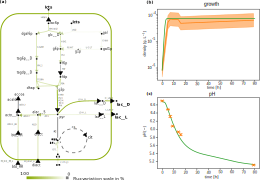
\includegraphics[width = 1\textwidth]{img/tango/FIG2_opt_explo_ll.pdf}
    \caption{\textbf{\lactis GEM fitted on pure culture data.} (a) FBA optimization with optimal parameters applied to the central carbon metabolism at the inoculation step. The color scale represents the reaction flux values predicted by the FBA and normalized by the highest flux value of the illustrated pathways. (b) Dynamics of \lactis population in pure culture after parameter inference in the model (green line) and in the experimental data (orange line, with $\pm 1/4$ log, which is the admitted range of precision for plating numbering). (c) pH in pure-culture of \lactis in the model (green line) and in the experimental data (orange crosses, with standard deviation). \textit{Compound abbreviations:} ac: acetate; actn\_\_R: acetoine; alac\_\_S: (S)-2-Acetolactate; btd\_RR: butanediol; cit: citrate; dgal6p: d-galactose-6-phosphate; dhap: Dihydroxyacetone phosphate; diact: diacetyl; f6p: fructose-6-phosphate; fdp: D-Fructose 1,6-bisphosphate; g1p: glucose-1-phosphate; g3p: Glyceraldehyde 3-phosphate; g6p: glucose-6-phosphate; gal: galactose; gal1p: galactose-1-phosphate; glc\_\_D: glucose; lac\_\_D, lac\_\_L: lactate; lac6p: lactose-6-phosphate; lcts: lactose; oaa: Oxaloacetate; pyr: pyruvate; tag6p\_\_D: D-tagatose-6-phosphate; tagdp\_\_D: D-Tagatose 1,6-biphosphate. \textit{Reaction abbreviations:} 6PGALSZ: 6-phospho-beta-galactosidase; ACLD: Acetolactate decarboxylase; ACTD2: Acetoin dehydrogenase; ACLDC: Acetolactate decarboxylase; ACLS: Acetolactate synthase; BTDD\_RR:  R R  butanediol dehydrogenase; CITL: Citrate lyase; CITt4\_1: Citrate transport via sodium symport; CS: Citrate synthase; D\_LACt2: D lactate transport via proton symport; ENO: Enolase; FBA: Fructose-bisphosphate aldolase; GAL6PI: Galactose-6-phosphate isomerase; GALkr: Galactokinase; GAPD: Glyceraldehyde-3-phosphate dehydrogenase; HEX1: Hexokinase (D-glucose:ATP); L\_LACt2r: L lactate reversible transport via proton symport; LACpts: Lactose transport via PEP:Pyr PTS; LACZ: B-galactosidase; LDH\_D: D-lactate dehydrogenase; LDH\_L: L-lactate dehydrogenase; PC: Pyruvate carboxylase; PFK: Phosphofructokinase; PFK\_2: Phosphofructokinase; PGI: Glucose-6-phosphate isomerase; PGK: Phosphoglycerate kinase; PGM: Phosphoglycerate mutase; PYK: Pyruvate kinase; TGBPA: Tagatose-bisphosphate aldolase; UGLT: UDPglucose--hexose-1-phosphate uridylyltransferase}
    \label{dfba_metabolite_lactis}
\end{figure}

\begin{figure}[htpb!]
    \centering
    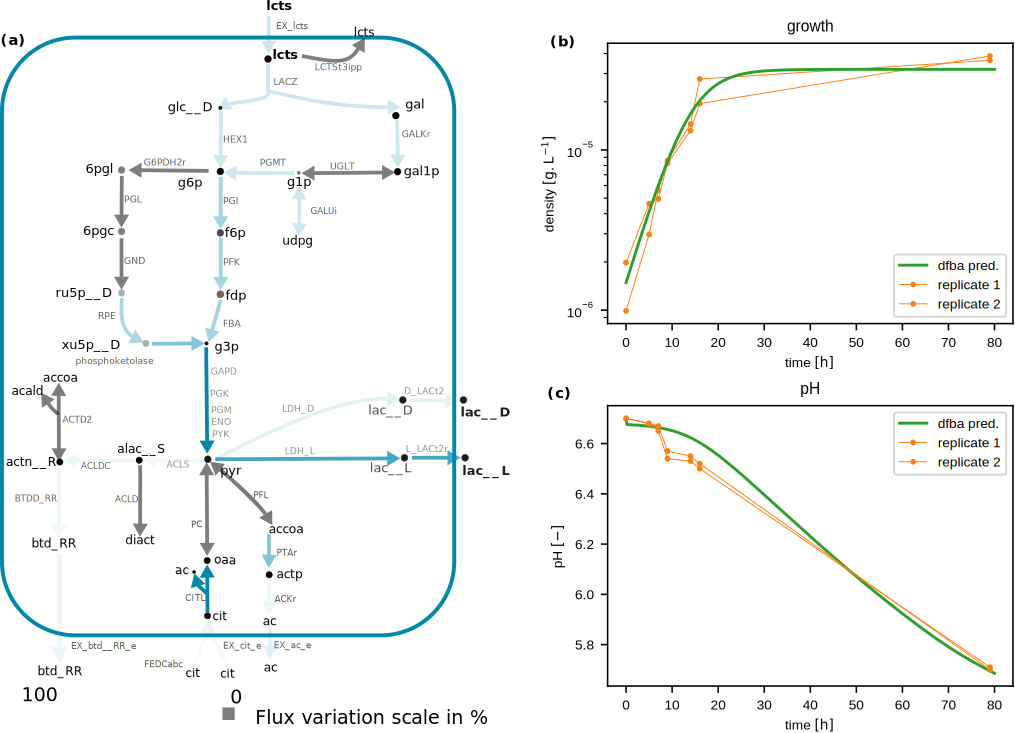
\includegraphics[width = 1\textwidth]{img/tango/FIG3_opt_explo_lp.pdf}
    \caption{\textbf{\plantarum GEM fitted on pure culture data.} (a) FBA optimization with optimal parameters applied to the central carbon metabolism at the inoculation step. The color scale represents the reaction flux values predicted by the FBA and normalized by the highest flux value of the illustrated pathways. (b) Dynamics of \plantarum population in pure culture after parameter inference in the model (green line) and in the experimental data (orange line, with $\pm 1/4$ log, which is the admitted range of precision for plating numbering). (c) pH in pure-culture of \plantarum in the model (green line) and in the experimental data (orange crosses, with standard deviation). 6pgc: 6-Phospho-D-gluconate; 6pgl: 6-phospho-D-glucono-1,5-lactone; ac: acetate; acald: acetaldehyde; accoa: acetyl-coa; actn\_\_R: acetoine; alac\_\_S: (S)-2-Acetolactate; btd\_RR: butanediol; cit: citrate; dhap: Dihydroxyacetone phosphate; f6p: fructose-6-phosphate; fdp: D-Fructose 1,6-bisphosphate; g1p: glucose-1-phosphate; g3p: Glyceraldehyde 3-phosphate; g6p: glucose-6-phosphate; gal: galactose; gal1p: galactose-1-phosphate; glc\_\_D: glucose; lac\_\_D, lac\_\_L: lactate; lcts: lactose; oaa: Oxaloacetate; pyr: pyruvate; ru5p\_\_D: D-Ribulose 5-phosphate; tag6p\_\_D: D-tagatose-6-phosphate; tagdp\_\_D: D-Tagatose 1,6-biphosphate; udpg: UDPglucose; xu5p\_\_D: D-Xylulose 5-phosphate. \textit{Reaction abbreviations:} ACLD: Acetolactate decarboxylase; ACTD2: Acetoin dehydrogenase; ACLDC: Acetolactate decarboxylase; ACLS: Acetolactate synthase; BTDD\_RR:  R R  butanediol dehydrogenase; D\_LACt2: D lactate transport via proton symport; ENO: Enolase; FBA: Fructose-bisphosphate aldolase; FEDCabc: FEDCabc; G6PDH2r: Glucose 6-phosphate dehydrogenase; GALkr: Galactokinase; GALUi: UTP-glucose-1-phosphate uridylyltransferase (irreversible); GAPD: Glyceraldehyde-3-phosphate dehydrogenase; GND: Phosphogluconate dehydrogenase; HEX1: Hexokinase (D-glucose:ATP); L\_LACt2r: L lactate reversible transport via proton symport; LACZ: B-galactosidase; LCTSt3ipp: Lactose transport via proton aniport (periplasm); LDH\_D: D-lactate dehydrogenase; LDH\_L: L-lactate dehydrogenase; PC: Pyruvate carboxylase; PFL: Pyruvate formate lyase; PTA: Phosphotransacetylase; PGL: 6-phosphogluconolactonase; PFK: Phosphofructokinase; PGK: Phosphoglycerate kinase; PGI: Glucose-6-phosphate isomerase; PGM: Phosphoglycerate mutase; PGMT: Phosphoglucomutase; phosphoketolase: phosphoketolase; PYK: Pyruvate kinase; RPE: Ribulose 5-phosphate 3-epimerase; UGLT: UDPglucose--hexose-1-phosphate uridylyltransferase.}
    \label{dfba_metabolite_plant}
\end{figure}

\begin{figure}[htpb!]
    \centering
    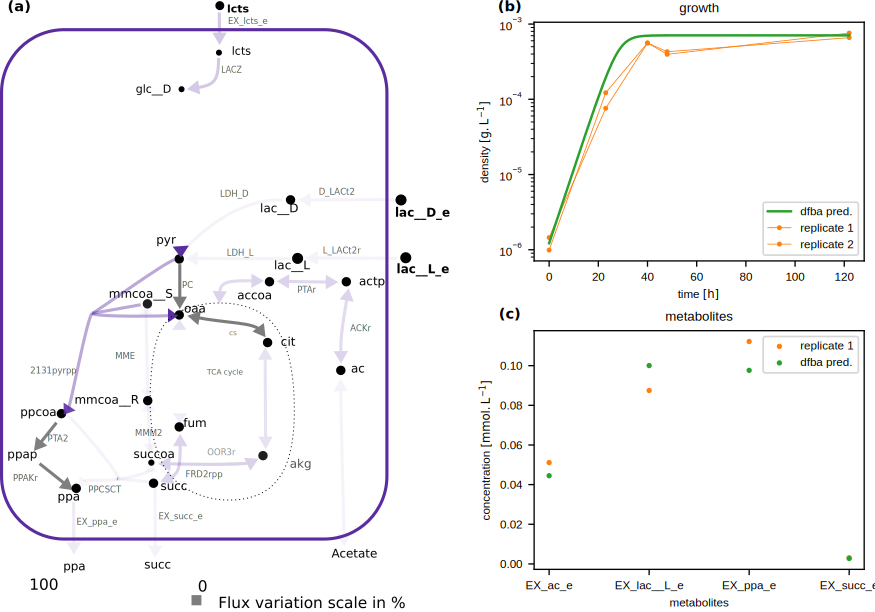
\includegraphics[width = 1\textwidth]{img/tango/FIG4_opt_explo_pf.pdf}
    \caption{\textbf{\freud GEM fitted on pure culture data.} (a) FBA optimization with optimal parameters applied to the central carbon metabolism at the inoculation step. The color scale represents the reaction flux values predicted by the FBA and normalized by the highest flux value of the illustrated pathways. (b) Dynamics of \freud population size in pure culture after parameter inference in the model (green line) and in the experimental data (orange line, with $\pm 1/4$ log, which is the admitted range of precision for plating numbering). (c) Lactate, acetate, propionate and succinate concentrations simulated (green points) and observed (orange crosses, with standard deviation) at the final time point of a second experiment with different lactate inoculation (see Material and method) \textit{Compound abbreviations : } ac: acetate;  akg: 2-Oxoglutarate; fum: fumarate; glc\_\_D: glucose; lac\_\_D, lac\_\_L: lactate; lcts: lactose; mmcoa\_\_R: (R)-Methylmalonyl-CoA; mmcoa\_\_S: (S)-Methylmalonyl-CoA; oaa: Oxaloacetate; ppa: propionate.; ppap: Propanoyl phosphate; ppcoa: propionyl-coa; pyr: pyruvate; succ: succinate; succoa: succinyl-coa.\textit{Reaction abbreviations :} 2131pyrpp : Methylmalonyl-CoA carboxyltransferase 5S subunit; CS : Citrate synthase; D\_LACt2 : D lactate transport via proton symport; FRD2rpp : Fumarate reductase / succinate dehydrogenase (irreversible) (periplasmic, membrane potential dissipating); L\_LACt2r : L lactate reversible transport via proton symport; LACZ : B-galactosidase; LDH\_D : D-lactate dehydrogenase; LDH\_L : L-lactate dehydrogenase; MME : Methylmalonyl-CoA epimerase; MMM2 : Methylmalonyl-CoA mutase; OOR3r : 2-oxoglutarate synthase (rev); PC : Pyruvate carboxylase; PPAKr : Propionate kinase; PPCSCT : Propanoyl-CoA: succinate CoA-transferase; PTA2 : Phosphate acetyltransferase.
    }
    \label{dfba_metabolite_freud}
\end{figure}

\subsection{Le suivie de la production des métabolites dans les conditions de co-cultures par le modèle de communauté}

Nous venons de voir tout le processus de curation et de calibration des modèles métaboliques individuels dans le but de prédire les concentrations et les croissances de co-culture ainsi que d'émettre de nouvelles interactions métaboliques au sein de ce consortium. Dans cette section, les données de co-cultures qui nous servirons de données tests à nos prédictions seront d'abord présentés brièvement, puis nous nous concentrons sur comment le modèle communautaire fut créé et son exploitation. 

Un suivi de la croissance des bactéries ainsi que de la production des metabolites ont été réalisé durant le fabrication du fromage. Chaque souche de ce consortium que sont \lactis, \plantarum et \freud ont atteint respectivement un seuil de culturabilité de 8.45 $\log_{10}$CFU/g, 8.47 $\log_{10}$CFU/g et 8.59 $\log_{10}$CFU/g en approximativement 1200 heures.

Pour vérifier si nous prédisons ces données, nous avons tout d'abord construit un modèle de communauté regroupant les modèles individuels calibrés où chaque individu maximise sa propre biomasse. Par la suite, nous avons ajusté la valeur du "quorum sensing", c'est à dire la valeur à laquelle nous observons une phase plateau, de chaque modèle individuel en intégrant la valeur des données expérimentales au sein de l'équation \ref{eq:logistic-growth} dans le but de reproduire le comportement métabolique de la communauté \textit{in silico} (voir eq.~\eqref{eq:system_dynamics_b}-\eqref{eq:system_dynamics_m} et matériels et méthodes \S\ref{sec:MandM-met-modelling}). Enfin, notons que, comme aucun ajustement du modèle de communauté n'a été fait, l'expérience de co-culture peuvent être considéré comme des données tests impliquant de nouveaux points de validations. 

Les prédictions à l'échelle de la communauté se font sur trois niveaux: croissance des bactéries, pH des bactéries lactiques, et métabolomique. Nous remarquons que le modèle de communauté prédit correctement  (Fig. \ref{dfba_community}(a)-(c), Table supplémantaire \ref{table:co-culture-data}). Nous remarquons cependant une légère surestimation de la croissance de \freud durant la phase exponentielle. Concernant la prédiction des métabolites issue de la métabolomique, nous observons une consommation plus lente du lactose tandis que celle du cirate s'ajuste bien avec les données expérimentales. La production de lactate est légerement surprédit durant la phase exponentielle résultant d'une légère suradification du fromage durant les étapes de moulage et de démoulage. En revanche, la production d'acétate est sous prédit durant les premières phases de la fabrication du fromage, mais le taux de production pendant la maturation est correctement modélisé. Les courbes du propionate, et dans une moindre mesure, celle du succinate sont prédit avec précision par le modèle suggérant que la production de composés organoleptiques par \freud est correctement capturée. De plus, les voies métaboliques activées en mono-cultures le sont également en co-culture (Figure \ref{fig:switch_metabolic_pathway}). Enfin, afin de valider statistiquement les prédictions du modèle communauté, nous avons fait une régression entre les valeurs prédites par le modèle et celles des données, et nous observons un $R^2$ globale de 0.98 pour cette étape de validation ( Figure \ref{fig:qqplot}, fenêtre de droite). Cela démontre que le temps passé sur la curation et le raffinement des modèles individuels, en combinant méthodes numériques et la connaissance biologique \textit{a priori} permet d'obtenir des prédictions à l'échelle d'une communauté avec une bonne précision. \\



\begin{figure}[htpb!]
    \centering
    \includegraphics[width = 1\textwidth]{img/tango/qqplot.pdf}
    \caption{\textbf{Model goodness of fit.} All the model outputs ($\hat{y}$) are plotted versus their respective data value ($y$) in the training (i.e. the mono-culture data, left panel) and in the testing set (i.e. the co-culture data, right panel). Each point is colored according to the data type and the bissector is plotted (red dotted line). A global coefficient of determination is computed with the formula $R^2 = 1 - \frac{\sum_i (y_i - \hat{y}_i)^2)}{\sum_i (y_i - \bar{y}_i)^2)}$, where $\bar{y}$ is the average value of $y$. We can observe a very good agreement of the model in the training set, and a globally good agreement in the testing set, with 3 outliers on lactose and citrate.}
    \label{fig:qqplot}
\end{figure}


\begin{figure}[htpb!]
    \centering
    \includegraphics[width=0.5\textwidth]{img/tango/supp_fluxes_pathways.pdf}
    \caption{\textbf{Metabolic pathway switches during cheese production.} For each bacterium we ran a dFBA simulation and reaction fluxes per each pathways of interest in Figure \ref{figure:metabolic_map} were retrieved at the inoculum of LAB (Linoc, t=0 hours), the inoculum of \freud (Finoc, t=18 hours the molding (Cm, t=19.5 hours), demolding (Cdm, t=40hours), start of ripening (C0w, t=60 hours), fourth week ripening (C4w, t=732 hours) and seventh week ripening state (C7w, t=1236 hours). We normalized fluxes by the inoculum flux value and the average flux for each pathways is therefore represented.}
    \label{fig:switch_metabolic_pathway}
\end{figure}

\begin{figure}[htpb!]
    \centering
    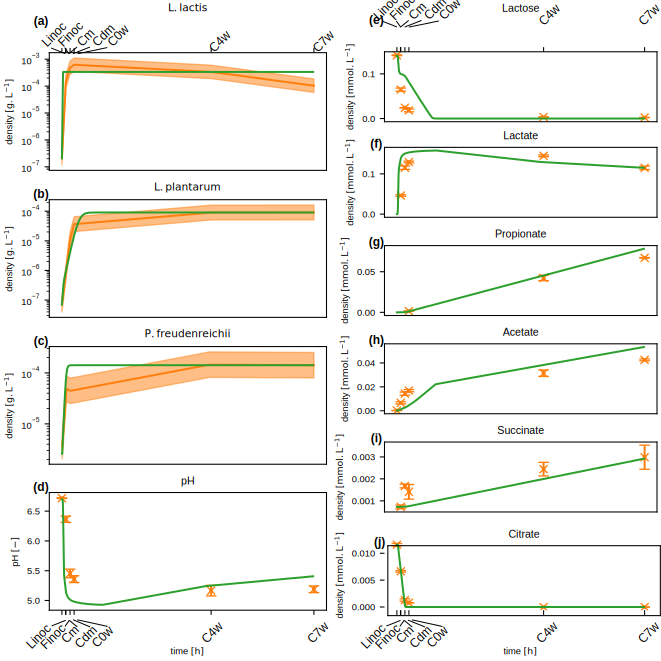
\includegraphics[width = 1.0\textwidth]{img/tango/Fig5.pdf}
    \caption{(a-c) Simulated growth of respectively \textit{L. lactis}, \textit{P. freudenreichii} and \textit{L. plantarum} species computed by the community model (green lines) and experimentally-observed (orange lines, confidence interval of $\pm$ 1/4 log). (d-j) Computational and experimental co-culture pH and metabolic profiles. Each data point is represented with its corresponding standard deviation (error bars). Abbreviations: Linoc, Lactic acid bacteria inoculation (t = 0); Finoc, \textit{P. freudenreichii} inoculation (t = 18 hours); Cm, molding (t = 19.5 hours); Cdm, demolding (t = 40 hours); C0w, start of ripening (t = 60 hours); C4w, Fourth week ripening (t = 732 hours); C7w, seventh week ripening (t = 1236 hours).}
    \label{dfba_community}
\end{figure}

\maxime{TODO : traduire les figure + retravailler paragraphe interactions}
\subsection{Les interactions bactériennes dynamiques au sein de la communauté}

Nous avons montré jusqu'à présent qu'associer la connaissance biologique, issu de la littérature et/ou d'un ou une biologiste, avec un modèle numérique est essentielle pour comprendre ce consortium bactérien du point du vue du métabolisme. De plus, notre avons montré que même un réseau métabolique de bonne qualité initialement nécessite une curation supplémentaire rigoureuse. En effet, l'utilisation de modèle suffisamment bien curé et raffiné a permis de reproduire les expériences biologique lors des simulations en communauté avec une bonne confiance dans les résultats. Grâce à cette assurance, nous pouvons exploiter d'avantage le modèle de communauté du point de vue des interactions bactériennes possibles au sein de cette communauté. Dans les paragraphes suivant, nous déduirons dans un premier temps des interactions que notre approche numérique a pu mettre en évidence en analysant les flux relatifs et absolu de production et de consommation de chaque métabolite pour chaque espèce. Dans un second temps, nous verrons ce que des outils sans connaissance \textit{a priori} peuvent découvrir. \\


Notre modèle numérique de communauté peut révéler des interactions microbiennes telles que l'alimentation croisée ou la compétition pour un nutriment. Dans ce but, nous nous sommes focalisés sur la dynamique des flux des métabolites d'intérêts pour chaque espèce (Fig. \ref{fig:flux-contrib}, (a)) en calculant, à chaque pas de temps de la dynamique, et à l'échelle de la population, les flux d'échange $\mu_{i,j} b_i$ pour chaque métabolite $j$ et bacterie $i$ et les concentrations des métabolites prédites associées. Concernant le lactose et le citrate, nous observons que \lactis les consomme très rapidement durant leur phase exponentielle avant d'être contrôlé par la régulation du pH pour le lactose et par la disponibilité du citrate. Nous pouvons observé que \plantarum ne contribue pas ou peu dans la consommation totale de ces métabolites suggérant ainsi que d'autres métabolites non suivie en dynamique sont utilisés pour la croissance de ce dernier, comme par exemple, les acides aminés. Une hypothèse pouvant expliquer ce phénomène peut être du à la croissance plus lente de \plantarum dans les premières heures du processus de production du fromage. En effet, on remarque que les processus de régulations sur la consommation du lactose et du citrate sont mis en jeu lorsque la densité bactérienne de \plantarum est encore faible. De manière surprenante, nous observons que \freud termine la déplétion du lactose à la place de \plantarum au tout début de la phase d'affinage, malgré que le lactose soit déjà produit. 

En effet, la production de lactate étant corrélée avec la consommation de lactose, nous observons une très forte production conduit par \lactis pendant deux cent cinquante heures, correspondant à l'affinage dans le processus de fabrication du fromage. En dépit d'une plus faible croissance de \plantarum, ce dernier contribue faiblement à la production de lactate également. Durant la phase de l'affinage, le lactate est consommé par \freud contribuant ainsi à à l'augmentation du pH dans la communauté comme obervé dans la Figure~\ref{dfba_community}~d. Originalement, nous remarquons que les trois souches bactériennes sont capables de produire de l'acétate dans le milieu extracellulaire où \lactis est encore le contributeur majeur suivi de \plantarum jusqu'au temps t = deux cents cinquantes heures, temps à laquelle leur phase plateau commence. Ce schéma est retrouvé chez les bactéries lactique intervant également dans la production du butanediol via la voie de l'acétolactate. Cependant, \freud continu de garder un taux de production constant d'acétate durant la maturation du fromage malgré la phase plateau atteinte. Enfin, le propionate et le succinate est produit à taux constant par \freud durant tout le processus d'affinage et seul la souche de \lactis est capable de produire le diacétyle jusqu'au debut de la période de l'affinage.


Afin d'obtenir la contribution en flux net de chaque souche au sein de ce consortium, nous avons intégré dans le temps la prédiction du FBA $\int_0^T \mu_{i,j}(t) b_i(t) dt$. Après normalisation de cet échange net par les échanges totaux au sein de la communauté (i.e. la somme des échanges net de chaque individu), nous avons obtenu les contributions de chaque souche pour chaque métabolite (Fig. \ref{fig:flux-contrib}, (b)). Ces contributions confirment que le succinate et le propionate sont uniquement produits par \freud, alors que le diacétyle (production) et le citrate (consommation) sont métabolisé par \lactis. \plantarum contribue à la production du butanediol, bien que le principale producteur est prédit comme pour être \lactis. Dans une moindre mesure, \lactis contribue plus que \plantarum à la production de l'acétate où cette dernière est dominée par \freud. En terme d'interaction bactérienne, on obserse une alimentation coisée pour le lactate entre \lactis (producteur) et \freud (consommateur). La consommation du lactose est partagé entre \lactis et \freud et curieusement, \freud commence la consommation après que \lactis arrête de le métaboliser, indiquant une segregation temporelle de l'utilisation de lactose, et pas de competition direct pour ce substrat.

Nous avons démontré ci-dessus que capturer la complexité des processus métabolique dans une communauté microbienne durant la fabrication de fromage requiert des considérations de la dynamique sous jacente au sein du système. Nous nous demandions si l'application d'approches computationelle \textit{a prioio} se reposant sur les modèles métaboliques à l'échelle du génome peuvent mettre en avant de nouvelles interactions putatives entre les souches. A cette fin, nous avons utilisé deux méthodes basé sur les flux, SMETANA \citep{Zelezniak2015} et MiCOM \citep{diener2020}, et une approche basé sur le raisonnement, Metage2Metabo \citep{Belcour.2020} dans le but de suggérer de nouvelle complémentarité métabolique au sein du consortium.

Les approches quantitative, MiCOM et SMETANA, ont mis en avant respectivement quatorze et vingt-cinq métabolites échangés (Table\ref{table:exchangeable-metabolites-MICOM} et \ref{table:exchangeable-metabolites-smetana}), alors que l'approche par raisonnement, Metage2Metabo, identifie onze métabolites qui ne peuvent pas être produits par une espèce sans interactions dans la communauté (Table supplémentaire \ref{table:added-value-M2M}). Une première observation est qu'un relativement grand nombre de métabolites sont en communs dans les prédictions des composés échangeables de SMETANA et MiCOM: lactate, qui est aussi prédit dans le modèle dynamique, phénylaalanine, serine, malate, succinate, xanthhine, H${_2}$S,2-ketoglutarate, glycollate et acetaldehyde. Les autres composés échangés prédit incluent principalement des acides aminés (isoleucine, proline, glycine, alanine). Pour chaque composé mis en avant par SMETANA nous avons utilisé les données metatranscriptomiques dans le but d'évaluer la validité des interactions les plus plausibles selon le score SMETANA (voir meteriels et methodes). Le H${_2}$S est prédit comme produit de \lactis et \plantarum et donné à \freud, le ribose est produit par \lactis et \plantarum et connommer par \freud, le glycerol produit par les bacteries lactiques et consommer par \freud) et enfin le phénylalanine produit uniquement par \plantarum et consommé par \freud. Pour chacun de ces métabolites prédits comme échangé, nous avons vérifié l'expression des gênes associés à la productions de ces métabolites chez les espèces donneurs, et à la consommation de ces métabolites chez les espèces receveuses (voir methodes et Figure supplementaire \ref{fig:heatmap_metaT}). Les résultats suggèrent que les interactions pour H${_2}$S, ribose et le glycerol sont plausibles à plusieurs étapes de la fabrication du fromage. A l'inverse, alors que les données d'expression de gènes montrent que les voies métaboliques de la consommation de la phénylalanine sont fortement exprimées chez \freud, leur production par \plantarum ne l'est pas, suggérant que cette interaction semble être moins recevable. Enfin, l'ensemble des métabolites dont la production est prédit par Metage2Metabo comme nécessitant des interactions dans la communauté inclus divers acides gras, comme galactose-1-phosphate, benzyl-Coa, Glyceraldehyde and xanthosine, indiquant une complementarité métabolique entre les souches.

\begin{table}[H]
\centering
\begin{adjustbox}{width=1.2\textwidth}
\begin{tabular}{|c|c|c|c|c|c|}
\hline
Bigg ID & Metacyc ID & Name & Metacyc Ontology & Export fluxes & Import fluxes\\
\hline
acald\_e	& ACETALD &	acetaldéhylde & Aldehydes-Or-Ketones, Aldehydes	& Pf; Ll &	Lp \\
akg\_e &	2-KETOGLUTARATE	& 2-oxoglutarate &	Acids, Organic-Acids	& Pf &	Lp \\
ala\_\_D\_e &	D-ALANINE &	D-ALANINE &	All-Amino-Acids, Acids, Amino-Acids, Organic-Acids	& Pf; Lp &	Ll \\
ala\_\_L\_e	& L-ALPHA-ALANINE &	L-ALPHA-ALANINE &	All-Amino-Acids, Acids, Amino-Acids, Organic-Acids	& Pf; Lp	& Ll \\
co2\_e &	CARBON-DIOXIDE	& CARBON-DIOXIDE	& Others, Others	& Pf; Ll &	Lp \\
coa\_e &	CO-A &	co enzyme A &	Groups, Others	& Pf; Ll	& Lp \\
fe2\_e	& FE+2	& Fe2+&	Ions, Inorganic-Ions, Cations &	Lp	& Pf; Ll \\
gly\_e	& GLY	& Glycine	& All-Amino-Acids, Acids, Amino-Acids, Organic-Acids &	Lp &	Pf; Ll \\
glyclt\_e &	GLYCOLATE &	GLYCOLATE	& Acids, Organic-Acids	& Pf &	Lp \\
gthox\_e &	OXIDIZED-GLUTATHIONE &	glutathione disulfide	& ORGANOSULFUR, All-Glutathiones &	Lp &	Ll \\
gthrd\_e	& GLUTATHIONE &	glutathione	& ORGANOSULFUR, All-Glutathiones, Thiols	& Ll	& Lp \\
h2o2\_e &	HYDROGEN-PEROXIDE &	hydrogen peroxide &	Peroxides, Others	& Ll &	Lp \\
h2o\_e	& WATER	& H2O	& Pseudo-Compounds, Others &	Pf; Ll	& Lp \\
h2s\_e	& HS	& hydrogen sulfide &	Ions, Anions, Inorganic-Ions	& Ll	& Lp; Pf \\
ile\_\_L\_e &	ILE &	isoleucine &	All-Amino-Acids, Acids, Amino-Acids, Organic-Acids &	Lp	& Pf; Ll \\
lac\_\_D\_e &	D-LACTATE &	d-lactate &	Acids, Organic-Acids	& Pf &	Ll; Lp \\
lac\_\_L\_e &	L-LACTATE &	l-lactate &	Acids, Organic-Acids &	Ll	& Lp; Pf \\
mal\_\_L\_e &	MAL	& malate &	Acids, Organic-Acids	& Pf; Lp &	Ll \\
nh4\_e &	AMMONIUM &	ammonium &	Ions, Inorganic-Ions, Cations	& Lp	& Pf; Ll \\
phe\_\_L\_e &	PHE &	phenylalanine &	Aromatics, All-Amino-Acids, Acids, Amino-Acids, Organic-Acids, Organic-aromatic-compounds &	Pf	& Lp \\
pro\_\_L\_e &	PRO &	proline &	All-Amino-Acids, Acids, Amino-Acids, Organic-Acids &	Ll	& Pf \\
ser\_\_D\_e &	D-SERINE &	serine	& All-Amino-Acids, Acids, Amino-Acids, Organic-Acids &	Ll	& Lp; Pf \\
ser\_\_L\_e &	SER	& serine &	All-Amino-Acids, Acids, Amino-Acids, Organic-Acids &	Ll &	Lp; Pf \\
succ\_e &	SUC	& succinate	& Acids, Organic-Acids &	Ll &	Pf \\
xan\_e &	XANTHINE &	xanthine &	Others, Others &	Ll	& Lp; Pf \\
 \hline
\end{tabular}
\end{adjustbox}
\caption{\textbf{Exchangeable metabolites highlighted by MICOM on the cheese bacterial community.} Abbreviations: Ll, \lactis; Lp, \plantarum, Pf, \freud}
\label{table:exchangeable-metabolites-MICOM}
\end{table}

\begin{table}[H]
\centering
\begin{adjustbox}{width=1.2\textwidth}
\begin{tabular}{|c|c|c|c|c|c|}
\hline
Bigg ID & Metacyc ID & Name & Metacyc Ontology & Export fluxes & Import fluxes\\
\hline
acald\_e	& ACETALD	& acetaldéhylde	& Aldehydes-Or-Ketones, Aldehydes & \multicolumn{1}{c|}{{\begin{tabular}[c]{@{}l@{}}Pf \\ Pf \\ Lp \\ Ll \end{tabular}}}
& \multicolumn{1}{c|}{{\begin{tabular}[c]{@{}l@{}}Ll \\ Lp \\ Ll \\ Lp \end{tabular}}} \\
\hline
akg\_e &	2-KETOGLUTARATE	& 2-oxoglutarate &	Acids, Organic-Acids &\multicolumn{1}{c|}{{\begin{tabular}[c]{@{}l@{}} Lp \\ Pf  \end{tabular}}}
& \multicolumn{1}{c|}{{\begin{tabular}[c]{@{}l@{}} Pf \\ Lp \end{tabular}}} \\
\hline
fum\_e &	FUM	& fumarate &	Acids, Organic-Acids &\multicolumn{1}{c|}{{\begin{tabular}[c]{@{}l@{}}Pf \end{tabular}}}
& \multicolumn{1}{c|}{{\begin{tabular}[c]{@{}l@{}}Lp \end{tabular}}} \\
\hline
glyc\_e &	GLYCEROL &	GLYCEROL &	Alcohols, All-Carbohydrates, Sugar-alcohols, Carbohydrates &\multicolumn{1}{c|}{{\begin{tabular}[c]{@{}l@{}}Lp \\ Ll \\ Ll \end{tabular}}}
& \multicolumn{1}{c|}{{\begin{tabular}[c]{@{}l@{}}Pf \\ Pf \\ Lp \end{tabular}}} \\
\hline
glyclt\_e &	GLYCOLATE &	GLYCOLATE &	Acids, Organic-Acids &\multicolumn{1}{c|}{{\begin{tabular}[c]{@{}l@{}} Lp \end{tabular}}}
& \multicolumn{1}{c|}{{\begin{tabular}[c]{@{}l@{}} Pf \end{tabular}}} \\
\hline
h2s\_e	& HS	& hydrogen sulfide &	Ions, Anions, Inorganic-Ions &\multicolumn{1}{c|}{{\begin{tabular}[c|]{@{}l@{}}Lp \\ Pf \\ Ll \end{tabular}}}
& \multicolumn{1}{c|}{{\begin{tabular}[c]{@{}l@{}}Pf \\ Lp \\ Lp \end{tabular}}} \\
\hline
lac\_\_D\_e &	D-LACTATE	& d-lactate &	Acids, Organic-Acids &\multicolumn{1}{c|}{{\begin{tabular}[c]{@{}l@{}}Pf \\ Ll \end{tabular}}}
& \multicolumn{1}{c|}{{\begin{tabular}[c]{@{}l@{}}Lp \\ Lp \end{tabular}}} \\
\hline
lac\_\_L\_e &	L-LACTATE &	l-lactate &	Acids, Organic-Acids &\multicolumn{1}{c|}{{\begin{tabular}[c]{@{}l@{}} Ll \end{tabular}}}
& \multicolumn{1}{c|}{{\begin{tabular}[c]{@{}l@{}}Lp \end{tabular}}} \\
\hline
mal\_\_L\_e &	MAL	& malate &	Acids, Organic-Acids &\multicolumn{1}{c|}{{\begin{tabular}[c]{@{}l@{}}Pf \\ Lp \\ Pf \\ Ll \end{tabular}}}
& \multicolumn{1}{c|}{{\begin{tabular}[c]{@{}l@{}} Ll \\ Ll \\ Lp \\ Lp \end{tabular}}} \\
\hline
phe\_\_L\_e &	PHE	& phenylalanine &	\multicolumn{1}{c|}{{\begin{tabular}[c]{@{}l@{}} Aromatics, All-Amino-Acids, Acids, Amino-Acids \\Organic-Acids, Organic-aromatic-compounds \end{tabular}}}   &\multicolumn{1}{c|}{{\begin{tabular}[c]{@{}l@{}}Lp  \end{tabular}}}
& \multicolumn{1}{c|}{{\begin{tabular}[c]{@{}l@{}}Pf \end{tabular}}} \\
\hline
rib\_\_D\_e &	D-Ribopyranose &	D-Ribopyranose &	Aldehydes-Or-Ketones, All-Carbohydrates, Aldehydes, Carbohydrates &\multicolumn{1}{c|}{{\begin{tabular}[c]{@{}l@{}}Ll \\ Lp \\ Pf \\ Ll \end{tabular}}}
& \multicolumn{1}{c|}{{\begin{tabular}[c]{@{}l@{}}Pf \\ Pf \\ Lp \\ Lp \end{tabular}}} \\
\hline
ser\_\_D\_e	& D-SERINE	& serine &	All-Amino-Acids, Acids, Amino-Acids, Organic-Acids &\multicolumn{1}{c|}{{\begin{tabular}[c]{@{}l@{}}Ll \\ Lp
 \\ Pf \\ Lp \\ Pf \\ Ll\end{tabular}}}
& \multicolumn{1}{c|}{{\begin{tabular}[c]{@{}l@{}} Pf \\ Pf \\ Ll \\ Ll \\ Lp \\ Lp \end{tabular}}} \\
\hline
succ\_e &	SUC &	succinate &	Acids, Organic-Acids &\multicolumn{1}{c|}{{\begin{tabular}[c]{@{}l@{}}Ll \\ Lp \end{tabular}}}
& \multicolumn{1}{c|}{{\begin{tabular}[c]{@{}l@{}}Pf \\ Pf   \end{tabular}}} \\
\hline
xan\_e &	XANTHINE &	xanthine &	Others, Others &\multicolumn{1}{c|}{{\begin{tabular}[c]{@{}l@{}}Ll \\ Lp \end{tabular}}}
& \multicolumn{1}{c|}{{\begin{tabular}[c]{@{}l@{}}Pf \\ Pf   \end{tabular}}} \\
\hline
\end{tabular}
\end{adjustbox}
\caption{\textbf{Exchangeable metabolites highlighted by SMETANA on the cheese bacterial community.} Abbreviations: Ll, \lactis; Lp, \plantarum, Pf, \freud}
\label{table:exchangeable-metabolites-smetana}
\end{table}


\begin{table}[H]
\centering
\begin{adjustbox}{width=1.2\textwidth}
\begin{tabular}{|c|c|c|c|}
\hline
Bigg ID & Metacyc ID & Name & Metacyc Ontology  \\
\hline
galt1p&	D-galactose-1-phosphate&	a D-galactopyranose 1-phosphate	&All-Carbohydrates,Carbohydrates\\
benzcoa&	BENZOYLCOA&	benzoyl-CoA&	Esters,Thioesters\\
xtsn&	XANTHOSINE&	XANTHOSINE	&\begin{minipage}[t]{0.8\linewidth}Organic-heterocyclic-compound,All-Nucleosides,Nitrogen-Molecular-Entities,Organic-heteromonocyclic-compounds,Organic-Heteropolycyclic-Compounds,Organonitrogen-Compounds,Nucleosides\end{minipage}\\
glyald&	GLYCERALD&	glyceraldehyde	&Aldehydes-Or-Ketones,All-Carbohydrates,Aldehydes,Carbohydrates\\
3hocoa&	ø	&	ø	&	ø\\
3hhdcoa	&CPD0-2232	&(S)-3-hydroxyhexadecanoyl-CoA	&Thioesters,Esters\\
3hdcoa&	CPD0-2244	&(S)-3-hydroxydecanoyl-CoA	&Thioesters,Esters\\
3odcoa&	CPD0-2123&	3-oxodecanoyl-CoA	&Thioesters,Esters\\
3hhcoa&	OH-HEXANOYL-COA	&(S)-3-hydroxyhexanoyl-CoA&	Thioesters,Esters\\
udcpp&	UNDECAPRENYL-P	&all-trans-undecaprenyl phosphate	&Lipids,Polyisoprenoids\\
3oocoa&	CPD0-2106&	3-oxooctanoyl-CoA	&Thioesters,Esters\\
 \hline
\end{tabular}
\end{adjustbox}
\caption{\textbf{Metabolites predicted to be producible through metabolic cross-feeding only by Metage2Metabo}}
\label{table:added-value-M2M}
\end{table}

\begin{figure}[htpb!]
    \centering
    \includegraphics[width = 0.6\textwidth]{img/tango/FigS2_heatmap.pdf}
    \caption{\textbf{Gene expression with metatranscriptomic data.} This heatmap displays the decile of the RPKM of gene transcript counts at a given time point (columns) and in a given micro-organism (the colored areas indicate to which bacteria the gene belongs). Then, the decile were color coded from highest deciles (dark red, highest expression in this micro-organism at this time point) to lowest decile (light red, low expression). The displayed genes were manually selected from the list of possible interactions raised by SMETANA: for a selected interaction metabolite, genes involved in production (in the donor), and in consumption (in the receiver) were retained for analysis. Selected interaction metabolites were $H2S$, ribose and phenylalanine. Additionally, genes involved in lactose consumption were added to this list. Abbreviations: Cm, molding (t = 19.5 hours); Cdm, demolding (t = 40 hours); C0w, start of ripening (t = 60 hours); C4w, Fourth week ripening (t = 732 hours); C7w, seventh week ripening (t = 1236 hours). }
    \label{fig:heatmap_metaT}
\end{figure}


\begin{figure}[htp!]  
    \centering
        \includegraphics[width = 1.0\textwidth]{img/tango/Fig6.pdf}
        \caption{(a) \textbf{Consumption and production flux dynamics.} We represent for each bacterium the dynamics of the consumption and production fluxes of the followed-up metabolites (colored plain lines). We also represent the dynamics of the concentration of the corresponding metabolite in the cheese (dashed black line, right axis for scale). (b) \textbf{Bacterial relative contribution to the metabolite fate.} We represent the relative contribution of each bacteria to the final metabolite concentration. Namely, we computed each microbial overall contribution by integrating in time its consumption or production flux ($\int_0^t \mu_{i,j} b_i$ for metabolite $j$ and bacteria $i$, see eq.\ref{eq:system_dynamics_m}), and normalized the result by the sum over the three bacteria. The value 1 (or -1) then represents the net production (or consumption), i.e. the difference between the final and initial concentration of the metabolite (horizontal dashed lines). For each metabolite, the bacterial contribution is represented by a colored bar, with positive value for production, and negative value for consumption. Abbreviations: Linoc, Lactic acid bacteria inoculation (t = 0); Finoc, \textit{P. freudenreichii} inoculation (t = 18 hours); Cm, molding (t = 19.5 hours); Cdm, demolding (t = 40 hours); C0w, start of ripening (t = 60 hours); C4w, Fourth week ripening (t = 732 hours); C7w, seventh week ripening (t = 1236 hours).}
        \label{fig:flux-contrib}
    \end{figure}
    
\newpage    

\section{Discussion}

Dans ce travail, nous fournissons un modèle de jumeau numérique du métabolisme bactérien pendant le processus de fabrication de fromage. En utilisant les modèles métaboliques de trois souches bactérienns inoculées et des données omiques, we etions capable de reproduire, avec précision, les motifs de production de metabolites ainsi que la dynamique des populations bactériennes. Nous nous sommes reposés sur les conditions expérimentales de cultures pures pour calibrer les modèles métaboliques individuels avec peu de paramètres pour chaque, ainsi limitant la surévalutation  du modèle durant les simulations communautaires. Une originalité du modèle est sa capacité de prédire les dynamiques sur tout le procedé de fabrication du fromage (sept semaines). Notre travail soulève des hypothèses sur les voies métaboliques mis en jeu dans le lait, ainsi que la contribution de chaque souche bactérienne dans la consommation de nutriments et la productibilité de composé organoleptiques.

La connaissance des microbiologistes, de la litérature scientifique et des données multi-omiques étaient nécessaire pour accomplire des modèles métaboliques à l'échelle du génome de grandes qualités et les simulations dynamiques qui en découlent. Le métabolisme carbonné central des bactéries lactiques produisent principalement l'acide lactique à partir de la dégradation du lactose \textit{via} les voies métaboliques de la glycolyse, du tagatose et de Leloir \citep{Widyastuti2014,VanRooijen1991,Kleerebezem2003}; pour la première fois, l'utilisation du citrate et de la fermentation hétérolactique ont été observé dans le modèle curé de \plantarum en lait. La vérification que chaque modèle métabolique individuel peut activer les différentes voies métaboliques décrites plus haut était ainsi une étape important pour valider les modèles, permettant la reproduction d'activités enzymatiques observé dans \citep{Quatravaux2006,Carroll1999}. La bactérie propionique \freud convertie le lactose, et préferenciellement le lactate en propionate selon \citep{Loux2015,Thierry2011}. En suivant \citep{Borghei2021}, nous avons ajouté l'enzyme propionyl-CoA:succinate Coa transferase (2.8.3.-) pour completer la cycle de Wood-Werkman, et ainsi assurer la production de propionate.

Dans \citep{Ozcan.2020}, les paramètres individuels de calibration pour tous les nutriements du milieu de culture sont imposés dans le but d'expliquer la métabolomique à l'échelle de l'espèce, et de les prédire à l'échelle de la communauté. En comparaison de ce travail, nous avons implémenté un modèle FBA dynamique en se basant sur \citep{Mahadevan.2002}, qui a utilisé des paramètres de calibration souche spécifique pour prédire la croissance, le pH et les concentrations métaboliques. Pour éviter la surévaluation du modèle, nous avons réduit le nombre de paramètres inférés pour chaque bactérie, où seulement deux paramètres sont gardés pour la régulations du pH pour les bactéries lactiques et un paramètre se focalisant sur les croissances de \plantarum et \freud. Des calibrations additionelles ont été mené pour \freud sans aucune optimisations mathématiques supplémentaires, en calculant la valeur de la borne supérieure des métabolites dosés en monoculture. 

Le modèle de co-culture a donné des indices sur le comportement de la communauté pendant la fabrication du fromage et a suggéré temporellement la contribution de chaque espèce impliqué dans la production des composés aromatiques. Il est montré que la production de propionate et d'acetate peut être attributé uniquement à \freud, comme indique dans \citep{Cao2021}, et que le diacetyl semble être seulement produit par \lactis. D'après le modèle de communauté, le butanediol a été produit pendant l'étape du moulage et au début de l'affinage par à la fois, \lactis et \plantarum, comme observé dans les modèles de mono-cultures respectifs. En regardant la production d'acétate, le modèle déduit une production précoce de l'étape du moulage jusqu'à l'affinage par \lactis et \plantarum suivi par \freud pendant l'affinage, responsable de la majeur partie de production de l'acétate à cette étape. Concernant l'utilisation des sources de carbonnes, alors que \plantarum possède les voies métaboliques de dégradation du lactose et du citrate, qui sont completement activées dans le modèle en monoculture, il apparaît que ces voies métaboliques sont fortement sous régulés en co-culture. Lors de la mise en culture avec \lactis, et comme la vitesse de croissance de \plantarum est la plus faible des deux, il accomplie son efficacité métabolique maximale après la phase exponentielle de \lactis. Comme \lactis pousse principalement sur le lactose produisant le lactate, sa phase exponentielle est associées à la forte acidification de milieu, ce qui active la régulation du pH par la répression du lactose sur le métabolisme de \plantarum. \plantarum peut utiliser des acides aminés ou d'autres métabolites non suivi par le modèle dynamique permettant sa croissance. Pour explorer cette piste, nous avons utilisé des outils dans le but d'identifier des interactions bacteriennes en dehors de l'ensemble des composés suivi par le modèle dynamique en co-culture, révélant d'autres interactions métaboliques putatives, où les acides aminés représentent une grande proportion.

Dans le modèle de co-culture, \freud garde activé son métabolisme dans la dernière phase de production d'un fromage : l'affinage. Ce métabolisme est reflété par la consommation de lactate durant tout l'affinage, et le relargage de composés organoleptiques à flux constant (Figure \ref{fig:flux-contrib}). Ce comportement est cohérent avec les capacités métaboliques connues de \freud et avec les données métabolomiques obtenu durant le procédé de production du fromage. Dans le modèle, \freud consomme aussi le lactose restantaprès la croissance de \lactis. En effet, durant sa phase exponentielle, \lactis metabolise principalement le lactose, produisant fortement du lactate et reduisant le pH. La réduction du pH inhibe l'absorption du lactose régulée par le pH dans les deux bactéries lactiques, et donc stoppant la consommation de lactose par les \textit{Lactobacilli}. Comme le lactose reste dans le milieu de culture et que \freud est l'unique bactéries capable de l'utiliser, il epuise donc le lactose encore présent. Dans les données métatranscriptomiques, le gêne LACZ est hautement activé par \freud durant l'affinage confirmant la dégradation du lactose par cette souche après l'acidification (Figure \ref{fig:heatmap_metaT}) 

Ce travail revèle comment la combinaison d'expert biologique, des données omiques et de la modelisation métabolique permet d'obtenir des prédictions précises sur les méchanismes responsable du comportement dynamique de la communauté microbienne. D'autre part, cela souligne également que la quantité de données et les efforts nécessaires pour créer de tels modèles de haute qualité restent un prix élevé à payer malgré l'amélioration des approches de simulation. Des développements méthodologiques doivent encore être proposés afin d'automatiser l'étalonnage des modèles avec des données et de garantir à la fois l'exactitude des prédictions et l'extensibilité à des communautés plus importantes ou à des communautés de composition empirique.


\section{Materiels et methodes}

\subsection{Données biologiques}

\subsubsection{Composition communauté.} Les souches qui ont utilisé dans le projet sont décrit dans \citep{Cao2021}. Brièvement, la communauté bacterienne controllé est composé de deux bactéries lactiques (LAB), \lactis subsp. \textit{lactis} biovar \textit{diacetylactis} CIRMBIA1206 (nommé \lactis), \plantarum CIRMBIA465 (nommé \plantarum), et une bactérie propionique \freud CIRMBIA122 (nommé \freud) provenant du Centre international pour les ressources microbiennes - Bactéries associées aux aliments (CIRM-BIA\footnote{\href{https://collection-cirmbia.fr/}{https://collection-cirmbia.fr/}})

\subsubsection{Fabrication de fromage et collecte des échantillons.} Le protocole standard de production d'un fromage décrit dans \citep{Cao2021} a été utilisé. Brievement, après la collect de lait frais, pasteurisé (\num{76}\unit{\degreeCelsius}, \num{20} \unit{secondes}), écrémer, standardisé (jusqu'à 30 grams de gras et 36 \unit{mg} de calcium par \unit{kg} de lait, \lactis et \plantarum sont inoculés a 5.7 et 5.2 log$_{10}$ \unit{CFU\per\gram} (Unité de Formant Colonie). Après pré-maturation du lait inoculé ( a \num{14} \unit{\degreeCelsius} pour \num{18} \unit{h}), \freud a été inoculé a 6.1 log$_{10}$ \unit{CFU\per\gram} et remué pendant \unit{20} \unit{min}. Le lait est versé dans des cuves et chauffé a \num{33}\unit{\degreeCelsius} pendant \num{30} \unit{min}. De la présure commerciale a été ajouté et le coagulum fut coupé, mélangé, lavé, drainé, pré-pressé et transféré dans des moules pour le présurage. Le demoulage apparait le troisième jour de la fabrication du fromage, et les fromages ont été salé (immersion a \num{12}\unit{\degreeCelsius} pendant \num{10}\unit{h} avec de la saumure en excès), puis séché toute la nuit et emballés sous vide dans des sacs en plastique le quatrième jour de la fabrication du fromage pour un affinage de  \num{7} \unit{weeks} à \num{13} \unit{\degreeCelsius}.

Après l'inoculation des bactéries lactiques (Linoc, t=\unit{h}) et de \freud (Finoc, t=18\unit{h}), les échantillons sont collectésà cinq etapes de production pour de plus amples analyses comme décrit dans \citep{Cao2021}: l'étape de moulage (Cm, t=19.5\unit{h}), l'étape de démoulage (Cdm, t=40\unit{h}), le commencement de l'affinage (C0w, t=60\unit{h}) après quatre et sept semaines d'affinage (C4w, t=732\unit{h} et C7w, t=1236\unit{h}). Les fromages sont répliqués quatre fois (des répétitions biologiques ont été réalisés à différents jours avec des incolua et laits différents), et échantillonés chaque fois pour la numérations et la biochimie et deux fois (répétitions biologiques) for le séquençage ARN.

\subsubsection{Expériences de culture souche spécifique.} Dans le but de calibrer les modèles métaboliques, un jeu de données d'entrainement a été réalisés en utilisant les données expérimentales de chaque souche individuel. Ces croissances individuelles des trois bactéries fut réalisé dans un lait gras UHT (Delisse) en tube dans des conditions microaerobic, c'est à dire, sans secouer dans l'incubateur a  30\unit{\degreeCelsius}, avec deux réplicats. Pour \freud, le lait fut supplémenté en lactate (20 \unit{g\per\L}) et avec de la peptone caseine (10 \unit{g\per\L}). Une seconde expérience de croissance fut réalisé pour \freud dans le but de mesurer la concentration finale de metabolites (acetate, lactate, propionate, et succinate). \lactis fut inoculé a $1\times10^{6}$ et $4\times10^{6}$ \unit{CFU\per\g}, \plantarum a $3\times10^{6}$ and $6\times10^{6}$ \unit{CFU\per\g} et \freud a $1.4\times10^{7}$ et $9\times10^{6}$ \unit{CFU\per\g}. Les données de croissance en culture pure sont disponibles en Table \ref{table:pure-culture-data}.

\subsubsection{Données métatranscriptomiques.} Dix grammes de fromage ont été dispersé dans 90 grammes d'une solution de citrate de sodium à 2\% durant 1 minute à vitesse maximal suivie de 1 min à faible vitesse dans un stomacher (Humeau, Treillière, France) à température ambiante. Dix millilitres de la dispersion ont été centrifugés à 10000 grammes à 4\unit{\degreeCelsius} pendant cinq minutes. Les culots cellulaires ont été conservés à -80\unit{\degreeCelsius} pour l'extraction de l'ARN. Après décongélation, les échantillons ont été centrifugés à nouveau pendant 5 minutes à 4\unit{\degreeCelsius}, 10 000 grammes pour retirer le surnageant. Les culots cellulaires ont été suspendus dans 200 μL de tampon de lyse (50 mM Tris-HCl, 1 mM EDTA ; pH 8,0) 20 mg/g de lysozyme (MP Biomedicals, Illkirch, France) et 50 U/g de mutanolysine (Sigma, Saint Quentin Fallavier, France) et incubés pendant 30 min à 24\unit{\degreeCelsius}. Les suspensions ont ensuite été transférées dans des tubes de 2 mL contenant 50 mg de billes de zirconium (diamètre : 0,1 mm ; BioSpec Products, Bartlesville) et 50 μL de SDS (20 \%). Les échantillons ont ensuite été agités dans un Precellys Evolution (Bertin, Montigny-le-Bretonneux, France) pendant deux cycles de 40 s à 6500 rpm. L'ARN a ensuite été extrait des lysats cellulaires à l'aide de Qiazol et du kit RNeasy Mini (Qiagen) selon \citep{Falentin.2010} avec deux ou trois étapes de traitement ultérieur à la DNase (Dnase Rnase free, Ambion) selon les instructions du fabricant. L'intégrité de l'ARN (RIN) a été évaluée à l'aide d'un bioanalyseur Agilent 2100 (Agilent Technologies, Santa Clara, CA). Les concentrations d'ARN ont été quantifiées à l'aide de la quantification fluorométrique Qubit (Thermofisher, France). L'absence de contamination par l'ADN a également été vérifiée à l'aide du Qbit et du protocole de quantification de l'ADN conformement aux instructions du fabricant. 
Les échantillons d'ARN ayant une valeur RIN supérieure à 8, indiquant une bonne intégrité de l'ARN, ont été conservés pour la suite de l'analyse.

Les données métatranscriptomiques ont été obtenues à cinq étapes de la fabrication du fromage. Les librairies Illumina et le séquençage ont été réalisés par GeneWiz (Leipzig, Allemagne). Les lectures sont disponibles à l'ENA (Cambridge) sous le numéro d'accession ENA : PRJEB42478. Les lectures séquencées ont été découpées à l'aide de Trim Galore et mises en correspondance avec les génomes de référence à l'aide de Bowtie 2 \citep{Langmead.2009}. Aucune erreur d'appariement n'a été autorisée et seules les lectures correspondant à des séquences uniques ont fait l'objet d'une analyse plus poussée. Les lectures correspondant à chaque séquence codante ont été comptées à l'aide de HTSeq-count (-stranded=reverse, -a 0, -t CDS, -i db\_xref, -m union) \citep{Putri.2022}.

Les analyses statistiques ont été réalisées à l'aide du logiciel statistique R version 4.0.3 \citep{R2021}. Les données brutes de comptage de l'ARN-Seq ont été normalisées en deux étapes. Tout d'abord, un facteur d'échelle spécifique à l'espèce a été appliqué pour éliminer les biais de composition entre les bibliothèques. Pour chacune des trois espèces, elles ont été calculées en utilisant tous les gènes de l'espèce considérée et deux autres rangées pour l'autre espèce, calculées comme la somme des comptages attribués à chacune de ces deux autres espèces, en utilisant la méthode TMM (Trimmed Mean of M- Values) telle qu'implémentée dans le package edgeR version 3.32.1 \citep{Robinson2010}. Une étape supplémentaire de normalisation au sein de l'échantillon a été réalisée pour corriger la longueur des gènes et permettre la comparaison. Enfin, la moyenne des réplicats a été calculée.


\subsubsection{Métabolomiques ciblées.}  Les méthodes sont décrites dans \citep{Cao2021}. Brièvement, les sucres et les acides organiques dans les échantillons sont quantifiés en utilisant la chromatographie liquide à haute performance (HPLC). Les composés volatils sont analysés en utilisant l'extraction par sorption de l'espace de la tête (HS) et couplés à la chromatographie en phase gazeuse-spectrométrie de masse (GC-MS).

\subsection{Modelisation métabolique}

\subsubsection{Séquençage du génome.} Des culots cellulaires (équivalent a 1e$^{10}$ CFU) ont été obtenus par centrifugation pendant 10 minutes à 5000 g à partir de cultures de souches dans un milieu de bouillon. L'ADN fut extrait en utilisant le kit DNeasy midi (Qiagen) d'après le protocole décrit dans \citep{Falentin.2010}. Les génomes sont séquencés par Illumina NovaSeq 2 x 1500 pb et PacBio Sequel (Eurofins Genomics, Constance, Allemagne). Les génomes sont assemblés en utilisant Unicycler \citep{Wick2017a,Wick2017b} sur laplateforme bioinformatique Galaxy Genotoul (Toulouse, France). Les séquence génomiques sont intégrés sur la plateforme MicroScope hébergé au Genoscope (CEA, Evry, France) pour une annotation automatique selon \citep{Vallenet.2019}. Les génomes annotés sont disponibles a l'ENA (Cambridge) sous le numréo d'accession ENA: PRJEB54980.

\subsubsection{Reconstruction de modèle métaboliques à l'échelle du génome.} Les génomes bactériens individuels sont annotés functionnellement en utilisant la plateforme MicroScope \citep{Vallenet.2019} Les réseaux métaboliques à l'échelle du génomes sont par la suite reconstruits à partir de ces génomes annotés avec CarveMe \citep{Machado2018} version 1.4.1. Chaque modèle métaboliques à l'echelle du génome est poli en utilisant ModelPolisher \citep{Romer2016} qui améliore l'annotation en ajoutant des informations liés aux identifiants BIGG depuis la base de connaissances BIGG \citep{King2016}. La consistance de chaque modèle est vérifié avec MEMOTE \citep{Lieven.2020} à la fin de l'étape de polissage (\url{https://memote.io}). Le milieu nutritionel inclus le milieu minimal trouvé par CarveMe et les composé du lait (\url{https://ciqual.anses.fr/\#/aliments/19024/lait-entier-pasteurise}, où les acides aminés sont considérés en excès (fichier supplementaire 1).

\subsubsection{Analyse par équilibre des flux.} Un modèle métabolique à l'échelle du génomes (GEM) est reconstruit pour chaque souche en utilisant le réseaux métabolique et la composition nutritionelle, et analysé avec la méthode de l'analyse par équilibre des flux (FBA) \citep{Orth2010}. Le FBA calcule une distribution de flux optimal satisfaisant la stoechiométrie et la faisabilité biophysique donnant un maximum de biomass, en solvant le programme linéaire suivant : 

\begin{equation}
\label{eq:fba}
\text{trouver }v^* \in \R^{N_r} \text{ tel que }  v^*= \argmax_{\begin{array}{c} S.v=0 \\ v_{min}^{in} \leq v \leq v_{max}^{in} \\ v_{min}^{ex} \leq v \leq v_{max}^{ex}   \end{array}}   v_{growth}
\end{equation}

ou $v_{growth}$ est le flux de la reaction de biomasse de modèle, $S$ est la matrice stoechihometrique derivé du modèle métabolique, $v_{min}^{in}$  et $v_{max}^{in}$ (resp. $v_{min}^{ex}$  et $v_{max}^{ex}$) sont les valeurs minimales et maximales de flux intracellulaires (resp. exchangés) définissant les bornes de flux pour le vecteur de flux $v$ contenant $\R^{N_r}$dimension. Les ensembles de valeurs $(v_{min}^{in},v_{max}^{in})$ et $(v_{min}^{ex},v_{max}^{ex})$ dans les GEMs sont disponibles dans le matériel supplémentaire.

L'équation \eqref{eq:fba} définit alors, pour chaque bactérie $i$, la correspondance $\mu_{i}$ entre les vecteurs de contraintes sur les réactions d'échange définissant l'environnement nutritionnel et le flux optimal $v^*$ obtenu dans ce contexte nutritionnel.
\begin{equation}
\mu_{i}(v_{min}^{ex},v_{max}^{ex}) = v^*
\label{eq:mu-fba}
\end{equation}

Le problème d'optimisation FBA \eqref{eq:fba} fut résolu en utilisant CobraPy \citep{Ebrahim2013}version 0.17.1 utilisant l'ordre lexicographique pour garantir une solution unique \citep{gomez2014dfbalab}.

\subsubsection{Raffinement manuel des GEMs} Une étape de raffinement manuel fut réalisé pour tous les modèle pour assurer la bonne production de composés organoleptiques et l'activité des fonctions métaboliques d'intérêt au regard de la littérature. Les modifications sont récapitulées dans le matériels supplémentaire Table \ref{table:manual-refinement}. Comme les trois espèces sont micro-aerobique, la borne d'import de l'oxygène est défini comme la valeur minimal permettant la production de composés aromatiques.
\begin{table}[htp!]
\begin{adjustbox}{width=1\textwidth}
\begin{tabular}{|c|c|c|c|c|}
\hline
GEM & Reaction & Bound & Value & Justification \\
 \hline
 \TableBac{\lactis}{8} & \TableReac{ACTD2}{lower}{0}{upper}{0}{Allows the activation of the acetolactate pathway} \\
 \cline{2-5}
 & \TableReac{ACLDC}{lower}{0}{upper}{2}{Allows the activation of the acetolactate pathway}\\
 \cline{2-5}
 & \TableReac{ACLS}{lower}{2}{upper}{1000}{Allows the activation of the acetolactate pathway}\\
 \cline{2-5}
 & \TableReac{LACZ}{lower}{0.0006}{upper}{2}{Force the consumption of lactose}\\ 
 \hline
 \TableBac{\plantarum}{10} & \TableReac{PFL}{lower}{0}{upper}{0}{Permit the production of both isomers of lactate from lactose.} \\
 \cline{2-5}
 & \TableReac{LCTSt3ipp}{lower}{0}{upper}{0}{Leads the flux of lactose into the Glycolysis pathway}\\
\cline{2-5}
 & \TableReac{ACTD2}{lower}{0}{upper}{0}{Allows the activation of the acetolactate pathway}\\
 \cline{2-5}
 & \TableReac{GALUi}{lower}{-30}{upper}{10}{Permit the production of both isomers of lactate from lactose.}\\
 \cline{2-5}
 & \TableReac{ACLS}{lower}{2}{upper}{1000}{Allows the activation of the acetolactate pathway}\\
 \hline
 \TableBac{\freud}{14} & \TableReac{6PGALSZ}{lower}{0}{upper}{0}{Tagatose pathway was used} \\
 \cline{2-5}
 & \TableReac{XYLI2}{lower}{0}{upper}{0}{\begin{minipage}[t]{0.6\linewidth}Production of fructose from glucose instead of glucose-6-phosphate. Glycolysis was not activated\end{minipage}}\\
\cline{2-5}
 & \TableReac{POX2}{lower}{0}{upper}{0}{Regulate flux of acetate}\\
 \cline{2-5}
 & \TableReac{PPAKr}{lower}{0}{upper}{0}{Inhibit acetate over production}\\
 \cline{2-5}
 & \TableReac{LACZ}{lower}{0}{upper}{5}{Allow consumption of lactose}\\
  \cline{2-5}
 & \TableReac{PTAr}{lower}{-1000}{upper}{8}{Allow the appropriate ratio of acetate/propionate}\\
  \cline{2-5}
 & \TableReac{2131pyrpp}{lower}{8}{upper}{1000}{Allow the appropriate ratio of acetate/propionate}\\
\hline
\end{tabular}
\end{adjustbox}
\caption{\textbf{Manual refinement of the GEMs and corresponding justifications.} \label{table:manual-refinement}}
\end{table}

\subsubsection{Modélisation dynamique} Le comportement dynamique de chaque système de culture est calculé en utilisant la l'analyse par équilibre des flux dynamique (dFBA) \citep{Mahadevan.2002} en ajoutant des mécanismes dynamiques de la population. Notons $b=(b_i)$ pour $i \in \mathcal{B}=\{\lactis,\plantarum,\freud\}$ les densités de la population bactérienne, et $m=(m_j)_{1\leq j \leq N_m}$ la densité de composés métaboliques $N_m$ qui sont expérimentalement suivi, nous avons ainsi le système, pour $i\in \mathcal{B}$ et $1\leq j \leq N_m$
\begin{align}
    \label{eq:system_dynamics_b}
    \partial_t b_i& = \mathcal{R}_{i}(b_i) {\mu}_{i,i}\left((c^{ex}_{min,i},c^{ex}_{max,i})(b,m)\right) b_i  \\
    \label{eq:system_dynamics_m}
    \partial_t m_j &= \sum_{i \in \mathcal{B}} {\mu}_{i,j}\left((c^{ex}_{min,i},c^{ex}_{max,i})(b,m)\right) b_i 
\end{align}
où le terme ${\mu}_{i,i}$ est la composante correspondant au métabolite $j$ (ou à la biomasse $i$) de $\mu_i$, calculé à partir de \ref{eq:mu-fba} compte tenu de l'ensemble des contraintes $(c^{ex}_{min,i},c^{ex}_{max,i})(b,m)$. Ces constraintes dependent dynamiquement de l'état de la variable $b$ et $m$.

Le vecteur  $\mathcal{R}_{i}$ modélise un processus de régulation de la population sur la croissance de la population de manière phenomenologique avec le terme 
\begin{equation}
\label{eq:logistic-growth}
    \mathcal{R}_{i} = \lambda_i (1-\frac{b_i}{\beta_i}), \text{ for }i \in \mathcal{B} 
\end{equation}

où $\lambda_i$ est un poids et $\beta_i$ est la capacité de charge de la population, correspondant à la valeur de la phase plateau de chaque bacterie dans l'expérience. 

Pour un substrat $j$ et une modèle métabolique $i$, la bornes usuelles sont
\begin{equation} 
c^{ex}_{min,i,j} = max(-\frac{m_j}{\Delta t \sum_{i\in \mathcal{M}_j} b_i},v^{int}_{i,j}) \quad \quad c^{ex}_{max,i,j} = 0,
\label{eq:usual-consumption-limitation}
\end{equation}

où $\mathcal{M}_j$ est le sous ensemble de bactérie métabolisant $j$ and $\Delta t$ est une caractéristique temporelle du temps d'importation. Ces équations reflète le partage uniforme des ressources parmis les bactéries durant la fenêtre temporelle $\Delta t$. Quand les substrats sont en excès, le flux est limité par la limite d'import intrinsèque $v^{int}_{i,j}$.

Certains substrats et produits sont également régulés. En suivant l'approche de \citep{Ozcan.2020}, comme le métabolisme du lactose par les bactéries lactiques est regulé négativement par la forme non dissocié de l'acide lactique avec une décroissance exponentielle, pour $j=lcts\_e$ et $i \in \{\lactis, plantarum\}$, nous avons 

\[ c^{ex}_{min,i,j} = max(-\frac{m_{lcts_e}}{\Delta t*\sum_{i \in \mathcal{M}(lcts_e)} b_i},-\mu_{max,lcts}*10^{(-k_{lac}*\phi_{undiss})}-\mu_{min,lcts})\]  

où $k_{lac}$ correspond à la décroissance exponentielle, $\mu_{max,lcts}$ et $\mu_{min,lcts}$ sont les valeurs maximales et minimales et $\phi_{undiss}$ est une fonction calculant la concentration de la forme non dissocié de l'acide lactate à partir du lactate. Cette fonction $\phi_{undiss}$ est dérivée de l'équation de Henserson-Hasselbalch comme dans \citep{Ozcan.2020} et lit
\begin{equation}
\phi_{undiss}(m_{lac\_\_L\_e},m_{lac\_\_D\_e}) = \frac{m_{lac\_\_L\_e}+m_{lac\_\_D\_e}}{1+ 10^{c_1 * (m_{lac\_\_L\_e}+m_{lac\_\_D\_e})+c_2}}.
\label{eq:undissociated-lactate}
\end{equation}

Dans cette équation le terme $c_1 * (m_{lac\_\_L\_e}+m_{lac\_\_D\_e})+c_2$ est une approximation linéaire de $(pH-pKa)$, alors que les paramètres 
$c_1$ et $c_2$ sont inférés par une régression linéaire des données de co-culture. La production de lactate est régulée de la même manière, alors que la production d'acétate est régulé en fonction de la disponibilité en lactose. Voir matériel supplémentaire section \ref{sec:dynamics-bounds} pour une description detaillée et justifications des bornes dynamiques configurées sur les réactions d'échange.

Pour \freud, les bornes supérieures de productions sont évalué en calculant par le flux de production à partir des dosages de métabolites et des données de croissance dans les expériences de culture pure, en supposant un flux constant (voir le matériel supplémentaire \ref{sec:estimate-bounds-freud}).

La condition initiale, l'inoculum et l'environnement nutritionnel constitué des composés du lait, acides aminés et co-facteurs, a été défini comme spécifié dans \citep{Cao2021}, après conversion des unités (voir matériel supplémentaire pour la liste des métabolites). Une masse cellulaire de $0.33\times10^{-12}$ \unit{\gram \per CFU} a été appliqué pour la conversion d'unité de biomasse.

\subsubsection{Implementation numérique} Le système dynamique est résolu avec le schéma semi-implicit d'Euler. A chaque étape $n$, après le calcul de $F_j$ le flux total du composé $j$ comme défini par l'ensemble des GEMs, 

\[ F_j=\sum_{i \in \mathcal{B}} {\mu}_{i,j}\left((c^{ex}_{min,i},c^{ex}_{max,i})(b^n,m^n)\right) b_i \,,\]

nous calculons,

\begin{align*}
b_i^{n+1}& = b_i^n+\Delta t* F_{b_i} \\
m_j^{n+1}& = \begin{cases} m_i^n+\Delta t* F_{j} & \text{ si } F_j>0 \text{(cas explicit)}\\
m_j^n/(1-\Delta t * F_j/m_j^n) & \text{ sinon (cas implicit)}
\end{cases}
\end{align*}
Ce schéma garantie la positivité de la solution pour touts les temps.

Les problèmes dFBA \eqref{eq:system_dynamics_b}--\eqref{eq:system_dynamics_m} ainsi que les paramètres inférés sont résolu en créant un scipt Python et en utilisant les bibliothèques \texttt{numpy} v.1.19.5\citep{harris2020array}, \texttt{pandas} v.0.25.3 \citep{mckinney2010data}, and \texttt{scipy} v.1.5.3 \citep{mckinney-proc-scipy-2010}. Durant le dFBA, le FBA est résolu en utilisant l'ordre lexicographique défini \citep{Gomez2018}.

\subsection{Ajustement du modèle}

Pour ajuster les paramètres du modèle, nous avons adapté les équations \eqref{eq:system_dynamics_b}--\eqref{eq:system_dynamics_m} aux expériences de monocultures. Nous avons ensuite inféré les le vecteur de paramètre du modèle $\theta$ du résultat du modèle de dFBA en maximisant le logarithme de la ressemblance des données obervé en monoculture. Formellement, pour $i \in \{ \lactis,\plantarum \}$, nous avons minimisé la fonction coût suivante 

\begin{equation}
J(b_i,pH | \theta_i, b_{i,exp},pH_{exp} ) = \| \frac{\logten(b_i) - \logten(b_{i,exp})}{\sigma_{log,i,exp}} \|^2 + \alpha \|\frac{pH - pH_{exp}}{\sigma_{pH,exp}} \|^2 
\label{eq:optim_LAB}
\end{equation}

où $\sigma$ (resp. $\sigma_{log,i}$) est l'écart-type (resp. l'écart-type log transformé) des données correspondantes, et $\theta_i = (k_{lac},\mu_{max,lcts})$ si $i=\lactis$ et $\theta_i = (k_{lac},\mu_{max,lcts},\lambda_i)$ si $i=\plantarum$.
Pour \freud, la fonction coût est 

\begin{equation} 
J(b,m | \theta_i, b_{exp},m_{exp} ) = \| \frac{\logten(b) - \logten(b_{exp})}{\sigma_{log,b,exp}} \|^2 + \alpha \|\frac{m - m_{exp}}{\sigma_{m,exp}} \|^2 
\label{eq:optim_freud}
\end{equation}

où $m_{exp}$ est le dosage final d'acétate, lactate, propionate et succinate, et $\theta_i = (\lambda_i)$. Nous avons gardé le nombre de paramètres d'ajustement petit (deux paramètres pour \lactis, trois pour \plantarum et un pour \freud) pour éviter la sur prédiction. Les résultats d'optimisation sont présentés dans la Table \ref{table:parameter-value}.

\subsection{Inférence des interactions metaboliques}

Dans le but de prédire des échanges métaboliques comme ceux qui apparaissent dans le consortium microbien, MICOM v 0.32.0 \citep{diener2020} et SMETANA v1.2.0 \citep{Zelezniak2015} ont été utilisé sur l'environnement nutritionnel du lait. En plus, la prédiction d'une complémentarité métabolique entre les trois modèles métaboliques poussant dans le lait fut révélé avec Metage2Metabo v1.5.0 \citep{Belcour.2020}. Tous les métabolites prédit par les outils sont classés dans des catégories supérieures: les identifiants de la base de données Metacyc v25.5 \citep{Caspi2018} des composés BIGG ont été retrouvé et l'ontologie de ces composés ont été utilisé. La liste des composés prédit comme intervenant dans ue interaction d'alimentation croisé est disponible à la Table supplémentaire \ref{table:added-value-M2M}.

Un sous ensemble d'interaction bactérienne putative fut sélectionné parmi ceux prédit par SMETANA, selon son propre score avec un seuil choisi à 0.5. La pertinence des métabolites échangés sélectionné  fut vérifié en utilisant les données de métatrancriptomiques (RPKM et moyenne des réplicats). Pour chaque métabolite, les réactions de production (dans l'espèce productrice) et de consommation (dans l'espèce consommatrice) des métabolites fut extraites en utilisant l'association gene-proteine-reactions. Dans le but d'évaluer l'expression putative de ces gènes, les valeurs d'expressions ont été comparé à l'expression globale des gènes dans chaque espèce, séparé en quartiles.

\subsection{Visualisation et analyses statistiques}

Les figures ont été généré en utilisant \texttt{matplotlib} version 3.3.4 \citep{Hunter.2007}. Les cartes métaboliques des voies métaboliques ont été généré avec Escher \citep{King2015} pour Python v3.6.9 \citep{rossum2009} \footnote{https://escher.readthedocs.io/en/latest/escher-python.html}, après avoir lancé un FBA pour chaque modèle. Les flux des réactions d'intérêt pour chaque espèce ont été normalisé par la valeur de flux maximal des voix métaboliques ciblées de l'espèce correspondante. 

\subsection{Code et disponibilité des données}
Le code pour les simulation métaboliques et les modèles métaboliques sont disponibles dans \href{https://forgemia.inra.fr/tango/tango\_models}{https://forgemia.inra.fr/tango/tango\_models}. Les génomes des trois souches bactériennes et leurs annotations sont disponibles dans l'ENA sous le nunmero d'accession PRJEB54980. Les données métatranscriptomiques sont disponibles dans l'ENA sous le numéro d'accession PRJEB42478. Les génomes annotés, les lectures ARN et RPKM sont deposé dans \href{https://entrepot.recherche.data.gouv.fr/privateurl.xhtml?token=4bf01466-29dd-4d71-b25e-b775d9cc39dc}{https://entrepot.recherche.data.gouv.fr/privateurl.xhtml?token=4bf01466-29dd-4d71-b25e-b775d9cc39dc}. Le dosage biochemiques et métaboliques dont disponibles donc \citep{Cao2021}.


\section{Conclusion}
Nous avons décrit dans ce chapitre une méthodologique numérique à l'échelle de chaque individu qui permet de garantir des bons résultats lors du passage à l'échelle de la communauté. Pour rappel elle consistait tout d'abord en un raffinement de chaque modèle FBA individuel dans le but de vérifier si les flux métaboliques passent par les bonnes voies métabolique. Puis, une combinaison entre le processus de partage équilibré des ressources ainsi qu'un faible nombre de paramètres optimisés ont permis de reproduire les observations biologiques et d'émettre des nouvelles hypothèses sur des possibles interactions bactériennes. \\
Tout ce travail demande de la patience, notamment pour l'étape de curation des modèles et requiert une grande quantité de données, deux points difficilement applicables pour le criblage au débit de communautés microbiennes. Le chapitre suivant présente ainsi une méthode existante utilisable pour le criblage de communautés, permettant de s'abstenir des deux principales contraintes mis en avant dans ce chapitre, et son extension pseudo-quantitative.


\begin{comment}
    
    \subsection{TANGO description}
    
    \subsection{Idée du paragraphe}
    A partir de TANGO, je dois être capable de justifier l'utilisation de la modélisation logique et du besoin de d'inférer un modèle hybride pour l'étude de communauté bactérienne. Orienter le papier informatique, on doit voir une majoriuté d'informatique et non biologique.
    
    Les points forts des modèles numériques : 
    \begin{itemize}
        \item Explication phénomène biologique avec une précision numérique à la fois pour chaque organisme sur les métabolites produits, la croissance, l'environnement et à la fois en communauté.
        \item Prédire à différentes échelles (metabolites, croissance bacterienne et communautaire)
        \item Intégrer une dimension temporelle 
    \end{itemize}
    
    Les points négatifs des modèles numériques :
    \begin{itemize}
        \item Coût de calcul corrélé au nombre d'organisme et nombre de métabolites que l'on suit dynamique
        \item Précision peut être limité par les données en entrées, leur nombre et leur qualité.
    \end{itemize}

    \subsection{Qu'est ce que le projet TANGO}

    Il s'inscrit dans un projet industriel visant à améliorer les propriétés organoleptiques d'un fromage. Pour cela, 2 bactéries lactiques et 1 bactérie propionique ont été préalablement choisi et mis en culture. Le processus de production du fromage se repartie en plusieurs étapes comme suit : moulage, demoulage, saumurage et affinage. A ces différents pas de temps cinétiques, des prélèvements ont été fait permettant d'obtenir des données sur le dénombrement bactériens, la quantité de métabolites produits (données metabolomiques)  et des données d'expressions de gènes (métatranscriptomics).\\

    A partir de ces données et d'une experte, comment peut-on construire un modèle numérique intégrant et expliquant les observations ?


    \subsection{L'inférence de réseau métabolique à partir de génome}
    (il y a biensur à mettre avant comment on reconstruit des réseaux métaboliques, les différents moyens etc)

    \subsection{Modèles numériques basés sur les flux}
    \subsubsection{état de l'art}
    [.....]

    \subsection{Raffinement des modèles FBA}

    Après avoir reconstruit les modèles FBA de chaque bactérie, la première étape fut de vérifier si les modèles FBA reproduisent bien les ce qui est connu. Cette vérification se fait à différents nivaux : 
    \begin{itemize}
        \item Chaque modele individuel statiquement puis dynamiquement
        \item Du modele de communauté statiquement puis dynamiquement 
    \end{itemize}

    Le processus peut-être interprété comme suit (mettre une figure qui explique tout ça) : si une modification se fait au niveau des modèles individuels, alors tout doit être vérifié depuis les modèles FBA individuels, même si la modification à pour but d'améliorer les prédictions sur le modèle de communauté.



    \subsection{Optimisation de paramètres en culture pur}

    \subsection{Données disponibles}
    \begin{itemize}
        \item Génome annoté de chaque bactérie 
        \item Courbes de croissance et de pH associées à chaque espèce (entre 4 et 7 points)
        \item Littérature : Identification des molécules produites par chaque espèce
    \end{itemize}
    Ces données sont utilisées pour :
    \begin{itemize}
        \item Obtenir les réseaux métaboliques à l'échelle du génome
        \item Paramétrer le dFBA (extraire la concentration de bactérie au temps t=0, la concentration maximale atteinte par bactérie, le pH au temps t=0)
    \end{itemize}


    \subsubsection{\textit{L. lactis} case}
    \textit{L. lactis} is a LAB that consume lactose to produce l/d lactic acid thanks to the glycolisis pathway(\textbf{reference of the mecanism}). This problem could occurs (\textbf{oliveira et al,2005}) and could be resolve by constraint the PFL reaction (\textbf{badri et al,2019}, \textbf{Melchiorsen et al, 2001}). In this paper, I propose to regulate the LACZ reaction that use water and lactose to produce galactose and glucose, that is a precursor of the glycolisis. By regulating the import flux of lactose into the glycolisis at 0.01, \textit{L. lactis} is able to produce L-lactic acid (see allFBA.tsv in supplematary informations. This threshold is found thanks to FVA methods (\textbf{references FVA})

    \subsubsection{\textit{L. plantarum} case}
    As \textit{L. lactis}, \textit{L. plantarum} is also a LAB that consume lactose to produce both isomers of lactic acid with the glycolisis pathway. To achieve this mecanism, the PFL reaction is blocked and the GALUI reaction is now authorized to produce glucose-1-phosphate from glucose-6-phosphate (galactose pathway) (\textbf{Brenda, metacyc}. The PFL, that produce acetyl-coa and formate from pyruvate is well knew regulatory reaction in a metabolism of LAB (\textbf{quatraveaux et al, 2006}).

    \subsubsection{\textit{P. freudenreichii} case}
    \textit{P. freudenreichii} is a rennet bacteria that consume lactic acid to produce propionic acid (\textbf{references}). This species is also able to consume lactose but it is not his preferred carbon source. In this study, the metabolic network of \textit{P. freudenreichii} produced lactic acid. Thanks to FVA methods, production flux were led to the tagatose (6PGALSZ reaction), the maltose production from threalose (MTI reaction) and a glucose isomerase that produce fructose from glucose (XYLI2 reaction) instead of glucose-6-phophate thanks to a hexokinase reaction. LACZ flux is also constrained to 0.018 to force the consumption of the lactose sugar (mecanism strain specific)


    - O$_2$ import flux was tuned to 2\\
    - the flux from acetyl CoA to acetate (PTAR) was switched off forcing flux of acetyl-CoA through TCA and WWC to favour propionate production and inhibit acetate production. Alternative options would have been to switch off citrate lyase or pox2, but PTAR is the least expressed reaction among the three in the metatranscriptomic data and provide the best fit with known propionate/acetate production ratio during PF122 growth. \\
    - lacZ was set between 0.2 and 0.5 to give priority to lactate over lactose consumption.\\
    After parameter optimization, the metabolism of PF122 was in line/agreement with biological data. Model output generated a growth curve including a stationary phase X h, a biomass of XX g corresponding maximum population size of cell / g of milk.

    \subsection{Déroulement}
    \subsubsection{Du génome au modèle FBA}
    Reconstruction de réseaux métabolique avec carveME. Le milieu de culture utilisé pour le gapfilling correspond à l'union du milieu culture du lait et le milieu de culture minimal définit par carveME (M9). La fonction de biomass à été ajouté automatiquement par carveME.\\

    Construction et correction des modèles FBA. Cette étape consiste à comparer les métabolites consommés et produits en flux par mes modèles par rapport à la littérature. Des ajustement espèces spécifiques on du être fait (voir le fichier article/supplemantary.tex). Ces ajustements sont justifier par rapport à la littérature.

    \subsubsection{Implémentation du modèle dFBA}
    Il faut définir les concentrations des métabolites dans le milieu de croissance et les modifier selon si on souhaite effectuer des simulations à l'échelle du génome ou bien de la communauté. Les concentrations des composés d'intérêt, que sont le lactose, le lactate et le propionate, ont été prise de la publication d'Hélène. Pour une simulation en communauté, le lactose sera la source de carbone principale. Lactate et propionate  sont à 0. Au préalable, les concentrations prises ont du être ajuster à la bonne unité. \\

    Il faut définir les concentrations de bactéries à l'inoculation. Pour une simulation en communauté, les concentration ont été prise dans la publication d'Hélène. Pour les simulation à l'échelle de chaque génome, la . concentration à été déduite des expériences en culture pure en lait. Un ajustement des unités à également été nécessaire. \\

    On lance simulation à l'échelle de chaque génome puis en communauté. Le but est de vérifier que l'on retrouve : 
    \begin{itemize}
        \item Les métabolites qui doivent être produits et consommés par chaque espèce (son comportement en culture pur)
        \item Les métabolites en produits et consommés en communauté 
        \item Les interactions connues associées a cette communauté
    \end{itemize}
    Si cette étape de vérification est pas bonne, il faut re-vérifier les modèles FBA.

    \subsubsection{Faire correspondre les données simulées aux données expérimentales}
    Deux types de données expérimentales sont à disposition : croissance en culture pur en lait et ceux de Tango, en communauté. Il faut d'abord faire correspondre données simulées aux données expérimentales en culture pure avant de passer à la communauté. Trois paramètres ont été optimisés : 
    \begin{itemize}
        \item un paramètre lambda : régule les bornes d'import des composés d'intérêt et modifie ainsi la croissance de la bactérie 
        \item un paramètre death\_rate : permet de simuler la décroissance bactérienne dans les modèle FBA. 
        \item un paramètre thresh\_hdc : correspond à la concentration maximale atteinte par la bactérie lors de la phase plateau (simule le quorum sensing). 
    \end{itemize}

    Pour chaque paramètre, une valeur initiale doit-être choisi. Le thresh\_hdc à directement été pris des données en culture pure. L'optimisation se base sur la distance au carré entre les données simulés et les données expérimentales. Les nouvelles valeurs sont inférées dans le modèle dFBA espèce, puis en communauté. \\

    Sur le modèle de communauté avec les nouveaux paramètres, je récupère la dynamique des métabolites d'intérêts de communauté. Puis je compare les concentrations prédites par le modèle dFBA avec les concentrations des molécules d'intérêt issu de la métabolomique. Attention la encore aux unités. 

    \subsubsection{debuggage de l'optimisation}
    Lorsque l'on manipule des données multi-omiques et que l'on souhaite vérifier que nos données simulées expliquent les observations, les conversions d'unités et la calibration des états initiaux du modèle sont les points à vérifier en priorité. Par la suite, un résultat non satifaisant peut-etre expliqué par plusieurs choses et la résolution est le fruit d'aller retour entre la connaissance d'un.e expert.e et le.a modélisateur.rice:

    \paragraph{Courbes de pH} Une des difficultés rencontrées étaient l'ajustement de la courbe de pH associés à la concentration de lactate prédite par dFBA à la vraie courbe de pH des données expérimentales. Les principales questions concernaient le choix de la formule de pH : est ce que l'on prenait la forme dissocié de l'acide ou non (acide lactique ou lactate) ? La seconde interrogation se portait se l'impact du pH sur le métabolisme de l'espèce.  Est-ce le pouvoir acidifiant de la bactérie affecte sa croissance ou sa production de métabolites, ni l'un ni l'autre ou les deux ? Enfin, est ce qu'il est biologiquement possible d'approximer le pH observé avec la production de l'acide lactique ou le lactate ? Concernant la dernière interrogation, nous avons observé qu'approximer le pH de \textit{P. freudenreichii} avec sa production de propionate uniquement ou en ajoutant acétate, le pH simulé était soit très basique soit très acide. Cela était du notamment à la différence de concentration entre ces deux acides et que la faible acidification de \textit{P. freudenreichii} observé dans les données est causé par d'autres mécanismes de régulation compensant la production des acides propioniques et acétiques.

    \paragraph{Courbes de croissance}
    Comme chaque espèce possède sa propre vitesse de croissance et de consommation des nutriments, nous avons donc, dans un premier temps, choisi deux paramètres souches spécifiques, $\lambda$ et $\text{QS}$, modifiant toutes les bornes d'importation des nutriments ainsi que la densité bactérienne maximale à atteindre. Par la suite, alors que les courbes de croissances observés étaient corrélées avec les courbes de croissance simulé, nous avons constaté que la production du lactate par les bactéries lactiques n'étaient pas suffisantes pour permettre d'expliquer les données de pH observés. Pour résoudre ce phénomène, plusieurs choix étaient possibles : (1) le flux intracellulaire bifurquait dans une voie métabolique annexe (2) le flux de consommation du lactose était trop ou pas assez important. Dans l'explication (1), ce fut une des raisons qui déclencha la suite des modifications que les espèces lactiques ont subi. Chaque nouvelle modification subit une double validation par la littérature et à la fois par une experte biologique. Dans le cas (2), on observé une très grande quantité de lactate produit par les bactéries lactiques ce qui rend le milieu trop acide vis à vis des données. Nous avons alors découplé la régulation de la consommation du lactose en créant un paramètre $\lambda_{lactose}$ qui sera régulé par le pH environnement, i.e. la production de lactate. Comme nous modifions le FBA, la croissance lors du dFBA pouvait être impacté. Une étape d'optimisation des nouvelles valeures de $\lambda$ et $\text{QS}$ est faite systématiquement afin de vérifier le pouvoir explicatif des données observés par nos modèles. 


    \paragraph{Données acides}

    Un point de méthodologique supplémentaire fut nécessaire pour le bactérie propionique : \textit{P. freudenreichii}. Nous avons eut des données d'acide de \textit{P. freudenreichii} relatant les concentrations finales de l'acide propionique, du succinate, de pyruvate, lactate et d'acétate. Notre première idée consistait à utiliser le modèle FBA calibré pour prédire ces composés afin de valider le modèle. Une première approche naïve consistait à ne pas créer un paramètre $\lambda$ pour chaque composé et de laisser le modèle calibré prédire les composés. Cette première approche nous a permit de conclure que la calibration du modèle ne suffisait pas. Nous avons donc découplé
    le paramètre $\lambda$ un a un pour chaque composé. L'objectif était d'identifier les composés pouvant être régulés par une simple modification de la borne d'exportation de ceux nécessitant une curation plus approfondie. Les résultats nous montra qu'avec une modification des bornes, seul le lactate se calibre sur les données et les autres composés ne semblait pas être affecté. Deux explications à l'échelle du métabolisme étaient possibles : \textit{P. freudenreichii} utilisait une autre source de carbone pour produire ces composés ou bien, une bifurcation intracellulaire avait lieu. En combinant l'analyse de la variance des flux et la littérature, aucune des deux hypothèses ne se démarquaient. Cependant, il existe des valeurs de flux pour lequel nous observons qualitativement le comportement souhaité concernant les données acides.

    Concernant \textit{P. freudenreichii}, nous avons donc un bon fit sur les courbes de croissance en optimisant avec 3 paramètres d'optimisation : $\lambda$, $lactate_{lower}$ et $QS$. En revanche, la précision numérique souhaité pour les données d'acide n'est toujours pas satisfaisante, il faut donc ajouter des contraintes supplémentaires dans l'optimiseur. Nous avons testés (1) l'inférence de données \textit{a priori} dans l'optimiseur et s'en servir comme contrainte,  puis (2), une approche (2) \textit{agnostique}, plus traditionnelle et qui consistait à réduire l'écart entre les données observés et les données simulées. Dans l'approche (1), données d'apprentissage sont différentes de celle de test, on conserve donc un pouvoir prédictif important. En effet, nous savons que le ratio entre la quantité de propionate et la quantité d'acétate est de 3:1, nous avons contraint la fonction coût comme suit :
    \begin{align}
        mu * (log(ppa(T_f))-log(ac(T_f)-log(3))^2
    \end{align}

    %% Attention, vérifier au près de Simon, si les log étaient à l'interieur de la somme ou à l'extérieur de la somme. pas besoin car je ne fais pas de différence entre la simulé et l'observé.

    $mu$ est un coefficient de poids adaptant le compromis entre les données de croissance et les données acides. Nous avons ainsi fait varier $mu$ de 0.1 à 10000 avec un facteur 10. Nous avons pu constater quelques améliorations, comme l'observation de la production d'acétate et de propionate. les écarts étaient encore trop qualitatif et on en conclu donc que ce type de contrainte semble peu adapté à l'optimiseur et l'approche (2) fut appliquée. L'avantage est que l'on garde le même formalisme que pour le fit sur les courbes de croissance. En revanche, les données de croissances et les données d'acides ont pas été réalisé dans le même "batch" même si les conditions nutritives de croissances sont identiques. Nous avons donc ajouté à la fonction coût l'écart au temps T final, les concentrations des métabolites suivi dans les données acides : 

    \begin{align}
        mu * (log(ppa(T_f\_sim)-log(ppa(T_f\_obs)))^2
    \end{align}


    En somme, un simple modification de bornes peut avoir un impact sur les interactions de la bactéries avec les phénomènes physico-chimiques. 



    \paragraph{Communauté}

\end{comment}


\ifdefined\FromMain %
\else % 
  \end{document} %